\chapter{Robust Dynamic Experiments for the Precise Estimation of Respiration and Fermentation Parameters of Fruit and Vegetables}
\label{paper2}
This chapter has been submitted to PLOS computational biology.\footnote{\textbf{Strouwen, A.}, Nicolaï, B.M., Goos, P. Robust dynamic experiments for the precise estimation of respiration and fermentation parameters of fruit and vegetables. PLOS computational biology, submitted. }
\section*{Abstract}
Dynamic models based on non-linear differential equations are increasingly being used in many biological applications. Highly informative dynamic experiments are valuable for the identification of these dynamic models. The storage of fresh fruit and vegetables is one such application where dynamic experimentation is gaining momentum. In this chapter, we construct optimal $\oxy$ and $\coxy$ gas input profiles to estimate the respiration and fermentation kinetics of pear fruit. The optimal input profiles, however, depend on the true values of the respiration and fermentation parameters. Locally optimal design of input profiles, which uses a single initial guess for the parameters, is the traditional method to deal with this issue. This method, however, is very sensitive to the initial values selected for the model parameters. Therefore, we suggest a Bayesian experimental design approach to robustify our input profiles to the unknown values of the parameters.
\section{Introduction}
Model-based approaches are commonly used in the analysis, control and optimization of biological systems. These models rely on knowledge of physical, chemical and biological laws, such as mass balances, transport phenomena and reaction kinetics, and are often described by a system of non-linear differential equations, with inputs and outputs. So, often, the structure of a model can be determined from first principles. However, the model will generally also rely on parameters whose numerical values cannot be determined from physical laws. These parameters must then be inferred from experimental data before the model can be put to use. The experiments required to estimate these parameters are often laborious and cost prohibitive. It is therefore important to determine experimental conditions that are rich in information and thus allow a precise estimation of the unknown model parameters.
\\
\\
At present, the model parameters are often estimated from data collected using multiple experiments at various combinations of input levels, which are kept constant throughout each individual experiment. Even if an appropriate experimental design technique is used to reduce the number of experiments that have to be performed, the experimental effort remains considerable. Alternatively, experiments in which the inputs vary in time can be conducted. This has been shown to be a cost-effective way to generate a highly informative data set \parencite{versyck}. Such experiments are called dynamic. In optimal design of dynamic experiments, time-varying input profiles are constructed to optimize the information content of a single experiment.
\\
\\
The major challenge for experimental design for any non-linear model is the dependence of the optimal input profiles on the true values of the unknown model parameters, whose estimation is the primary goal of the experiment. This dependence is due to the non-linearity of the model. Most of the experimental design literature uses a scalar function of the Fisher information matrix as the measure of information content in an experiment, as this matrix is inversely related to the covariance matrix of the
model parameters. An informative experiment thus ensures a small covariance matrix of the model parameters. Locally optimal design of input profiles uses initial guesses for the model parameters to calculate this information matrix \parencite{fedorov}. This method has already been used to construct informative time-varying inputs in chemical engineering \parencite{franceschini} and in biological fields such as systems biology \parencite{balsa1}, predictive microbiology \parencite{bernaerts1,bernaerts2} and food engineering \parencite{balsa2,nahor}. However, an input profile that is highly informative for one set of parameter values may lack information for other parameter values. Thus, if the initial guesses of the parameters differs substantially from the true values, then the experiments might not allow precise parameter estimates. So, locally optimal design is sensitive to the initial parameter guesses and is thus not robust.
\\
\\
Much recent research in experimental design for non-linear models aims at robustifying the design to the true, but unknown, values of the model parameters. A robust design provides a large information content regardless of the true values of these parameters. For dynamic experiments, in particular, a min-max based approach has been used by \textcite{bauer, korkel}. Here, the design is optimized for a worst case scenario. Fisher information matrices are calculated for a set of possible parameter values and the experiment is scored based on the least informative matrix in this set. In contrast, an expected value approach is taken by \textcite{schenkendorf, telen, nimmegeers}. In this approach, the average information content of the experiments over all possible parameter values is optimized. The expected value approach tends to perform better for a large subset of probable parameter values than the min-max approach, but not for extreme sets of parameter values. The expected value approach is also called Bayesian experimental design, because the possible parameter values can be expressed using a prior distribution \parencite{chaloner}. The expected value approaches of \textcite{telen, nimmegeers} rely on  parametric distributions to describe the uncertainty on the model parameters before the experiment has taken place. However, for non-linear models, a parametric distribution will often not be appropriate to fully quantify the uncertainty on the model parameters. Therefore, in this chapter, we allow arbitrary distributions to quantify the model parameter uncertainty. More specifically, we show how the results of a Bayesian analysis of historical data using Markov-chain Monte-Carlo can be used as a prior distribution. This Markov chain can then be used to calculate the average Fisher information matrix, and has the advantage that it can represent arbitrary distributions \parencite{gelman}.               
\\
\\
Postharvest storage of fresh fruit and vegetables is one biological application where optimal experimental design is useful. The ideal storage temperature as well as $\oxy$ and $\coxy$ partial pressures depend on the respiration characteristics, which in turn depend on species, cultivar, ripeness and multiple other factors. Determining the ideal storage conditions therefore requires much experimentation. Traditionally, this was done by independently storing the product at many different combinations of temperature as well as $\oxy$ and $\coxy$ partial pressures, and by monitoring the respiration and fermentation \parencite{saltveit}. Many modern storage applications, such as modified atmosphere packaging \parencite{fonseca} and dynamic controlled atmosphere \parencite{bessemans}, adopt a model-based approach, where the product is described as a dynamic system with inputs and outputs. The resulting models enable us to use the tools of optimal dynamic experimental design to construct informative experiments. The respiration and fermentation kinetics are generally described by a model of the Michaelis-Menten type \parencite{hertog}. Robust experimental design is particularly needed for postharvest applications because of the large biological variability of fresh fruit and vegetables. As a consequence of that variability, the parameters of the aforementioned kinetic models vary substantially between seasons and origins. In this chapter, we therefore focus on constructing robust experimental techniques to estimate the respiration and fermentation kinetics of pear fruit. This chapter describes the first use of robust optimal experimental design techniques in postharvest research.
\\
\\
This chapter is structured as follows. First, in Section \ref{sec_OED}, we present our robust experimental design methodology. Next, in Section \ref{sec_pear}, we present a state of the art dynamic respiration and fermentation model for pear fruit, and quantify the initial uncertainty on the model parameters using a Markov-chain Monte-Carlo analysis of a prior data-set from \textcite{ho}. In Section \ref{sec_experiments}, we construct both locally and Bayesian optimal designs for this model. Finally, in Section \ref{sec_discussion}, we end with a discussion of alternative techniques we are planning to use in future work.
\section{Bayesian Optimal Experimental Design for Dynamical Systems}
\label{sec_OED}
In this section, we first present the type of dynamical models considered in this chapter. Then, we show how to quantify the information gained from measurements, using the Fisher information matrix. Next, we discuss how to maximize this information content using appropriate control inputs. Finally, we explain how to make the optimal control inputs robust.
\subsection{Dynamic Models}
In this chapter, we consider experimental design for dynamic models of the form:
\begin{equation}
\label{systemP2}
\begin{aligned}
\frac{\dd \bm x}{\dd t} &= f(t,\bm x,\bm \theta,\bm u(t)), \qquad \text{with } \bm x(t=0) = \bm x_0;\\
\bm y_k &= h(\bm x(t_k)) + \bm \epsilon_k,
\end{aligned}
\end{equation}
where $t$ denotes the time ranging from $0$ to $t_e$, the end time of the experiment. The column vector $\bm y_k$ contains the measurements taken at time point $t_k$, with $k$ ranging from $1$ to $N$, the number of measurement times. The time between measurements is equally spread, so that $t_k = \nicefrac{kt_e}{N}$. A measurement at the end of the experiment is thus included, but not at the start. The measurements are subject to independent zero mean Gaussian noise. More specifically,  $\bm \epsilon_k$ is identically and independently multivarate normally distributed with zero mean and covariance matrix $\bm R$. The measurements depend on the dynamic state column vector $ \bm x(t)$ through the measurement function $h$. The states $\bm x(t)$ have to be calculated from the system of ordinary differential equations $f$, with initial conditions $\bm x_0$. This system depends on the unknown model parameter column vector $\bm \theta$, and the controllable input column vector $\bm u(t)$.
\subsection{Information Content of an Experiment}
Our goal is to optimize the controllable inputs $\bm u(t)$ so that the measurements $\bm y_k$ contain as much information as possible about the unknown parameters $\bm \theta$. A popular way to quantify the information content is the Fisher information matrix (FIM) \parencite{fedorov, walter}:
\begin{equation}
\mathbb{F}(\bm \theta, \bm u(t))= \sum_{k=1}^N
\frac{\partial \bm x(t_k)}{\partial \bm \theta}^T
\frac{\partial h}{\partial \bm x}^T
\bm R^{-1}
\frac{\partial h}{\partial \bm x}
\frac{\partial \bm x(t_k)}{\partial \bm \theta}.
\label{FIM}
\end{equation}
The sensitivities of the states to the unknown parameters, $\nicefrac{\partial \bm x(t_k)}{\partial \bm \theta}$, cannot be computed directly, as the evolution over time of the states $\bm x(t)$ is described by the system of differential equations in Equation (\ref{systemP2}). However, these sensitivities can be calculated from the forward sensitivity differential equations:
\begin{equation}
\frac{\dd}{\dd t} \frac{\partial \bm x}{\partial \bm \theta}
=  \frac{\partial}{\partial \bm \theta}\frac{\dd \bm x}{\dd t}
= \frac{\partial f}{\partial \bm x}\frac{\partial \bm x}{\partial \bm \theta}
+ \frac{\partial f}{\partial \bm \theta},
\qquad \text{with } \frac{\partial \bm x(t=0)}{\partial \bm \theta} = \bm 0.
\label{sens}
\end{equation}
The FIM is the inverse of the Cramer-Rao lower bound of the variance of an unbiased estimator of $\bm \theta$. This lower bound can be interpreted geometrically as a hyper-ellipsoid defined by the eigenvectors and the inverse of the eigenvalues of the FIM. We want this lower bound to be as small as possible, and thus the eigenvalues of the FIM to be as large as possible, because this implies precise estimates for $\bm \theta$ are possible. In the literature, several scalar functions are used to quantify the size of the FIM \parencite{atkinson}. In our work, we use the determinant of the FIM, also called the D-optimality criterion. This criterion is inversely related to the volume of the hyper-ellipsoids, measuring the uncertainty about the parameter vector $\bm \theta$.
\subsection{Discretizing the Controls}
Optimal experimental design for dynamic systems is an infinite dimensional optimization problem since it requires finding optimal controls $\bm u(t)$ for every $t \in [0,t_e]$. To make this problem tractable, the controls have to be discretized in time. We utilize a bounded piecewise constant discretization allowing $\bm u(t)$ to switch values at $M$ equally spaced time points,
\begin{equation}
\bm u_{\min} \leq \bm u(t) = \sum_{j=1}^M \bm u_j \chi_{\left [\nicefrac{(j-1)t_e}{M},\nicefrac{jt_e}{M}\right [ }(t) \leq \bm u_{\max},
\label{input}
\end{equation}
where $\bm u_j$ is the constant control vector during the interval
$\left [\nicefrac{(j-1)t_e}{M},\nicefrac{jt_e}{M}\right [$, and $\chi_A$
is the indicator function,
\begin{equation}
\chi_A(t) =
\begin{cases} 1 \quad t\in A \\ 0 \quad t\not\in A, \end{cases}
\end{equation}
and $\bm u_{\min}$ and $\bm u_{\max}$ are the minimum and maximum control values allowed. Piecewise constant input profiles do not only have the benefit of making our optimization problem tractable, but they are also easy to implement in practice.
\subsection{Robustifying the Experiment}
Another issue with experimental design for models that are non-linear in the parameter vector $\bm \theta$, such as the model we described in Equation (\ref{systemP2}), is the dependence of the FIM on $\bm \theta$. This presents us with a cyclic problem because we are performing the experiment to quantify those parameters. Locally optimal experimental design is the traditional method to deal with this issue. In this approach, the FIM is calculated using a single initial guess $\bm \theta^*$ obtained from any available prior knowledge. A locally optimal experimental design is thus given by:
\begin{equation}
\argmax_{\bm u_1 \ldots \bm u_M} \quad \left | \mathbb{F}(\bm \theta^*, \bm u(t)) \right |
\qquad \text{subject to } \bm u_{\min} \leq \bm u(t) \leq \bm u_{\max}.
\label{localD}
\end{equation}
This method might give poor results if the initial guess deviates from the true value, and is thus not robust. Bayesian optimal design offers a solution to this robustness problem by averaging the information content of the experiment over multiple possible values of the parameters, taking into account the likelihood of each parameter value. More specifically, a weighted average is used to quantify the information content, where the weights are given by a prior distribution of the parameters $p(\bm \theta)$. This distribution represents the belief of uncertainty concerning these parameters, before the experiment has been performed. A robust experimental design is therefore given by:
\begin{equation}
\argmax_{\bm u_1 \ldots \bm u_M} \quad \int \left | \mathbb{F}(\bm \theta, \bm u(t)) \right | p(\bm \theta) \dd \bm \theta
\qquad \text{subject to } \bm u_{\min} \leq \bm u(t) \leq \bm u_{\max}.
\label{pseudoD}
\end{equation}
This criterion is also called the Bayesian D-optimality criterion \parencite{chaloner}, because of the use of a prior distribution.
\\
\\
Generally, the integral in Equation (\ref{pseudoD}) cannot be evaluated analytically. To approximate it numerically, we draw $R$ random model parameter vectors, $\bm \theta_r$, from the prior $p(\bm \theta)$ and average the D-criterion over these values:
\begin{equation}
\label{pseudoDcalc}
\quad \int \left | \mathbb{F}(\bm \theta, \bm u(t)) \right | p(\bm \theta) \dd \bm \theta
\approx \frac{1}{R} \sum_{r=1}^{R} \left | \mathbb{F}(\bm \theta_{r}, \bm u(t)) \right |
\qquad   \bm \theta_r \sim p(\bm \theta).
\end{equation}
The robust criterion in Equation (\ref{pseudoD}) is thus calculated by averaging the FIM over a sample drawn from the prior distribution. The details of the generation of this sample are explained in Section \ref{sec_markov}. 
\subsection{Numerical Details}
The entire optimization problem was implemented in the Julia programming language \parencite{bezanson}. 
All differential equations were solved using the Tsitouras 5/4 Runge-Kutta method \parencite{tsitouras}, as implemented in OrdinaryDiffEq.jl \parencite{rackauckas}. The piecewise constant control switches were implemented using a periodic callback, provided by DiffEqCallbacks.jl. Note that $\bm u(t_e)$ in Equation \ref{input} is undefined, but this value does not influence the FIM.
\\
\\
Because coding the sensitivity differential equations in (\ref{sens}) by hand is quite laborious and error prone, we calculated them exploiting the automatic differentiation capabilities of DiffEqSensitivity.jl \parencite{rackauckas2}, more specifically its implementation of the discrete forward sensitivity analysis method.
\\
\\
To solve the non-linear optimization problems, we used the box constrained optimization capacities of Optim.jl \parencite{mogensen}, which utilizes a log barrier interior point algorithm \parencite{nocedal}. This method requires the specification of an inner solver, for which we used the Broyden–Fletcher–Goldfarb–Shanno (BFGS) algorithm, as also implemented in Optim.jl. The required gradients for this method are calculated by the nested differentiation capabilities of ForwardDiff.jl \parencite{revels}. This interior point optimization method requires an initial experimental design to improve upon and is a local optimizer. Thus, it is not guaranteed to find the absolute best experimental design. To deal with this issue, we utilize multiple starts, each with a different initial design. The TikTak global optimization algorithm \parencite{arnoud} can carefully select these initial designs from the design space, using Sobol points. We use $1000$ starts of the interior point optimization method in combination with the TikTak implementation in MultiStartOptimization.jl.
\section{Respiration and Fermentation Model of Pear Fruit}
In this chapter, we apply our robust experimental design methodology to  precisely estimate the respiration and fermentation characteristics of pear fruit. First, we present a respiration and fermentation model of pear fruit inside a jar. We then quantify the initial uncertainty concerning the various parameters in this model using a published data-set.
\label{sec_pear}
\subsection{Model Description}
\begin{figure}
	\centering
	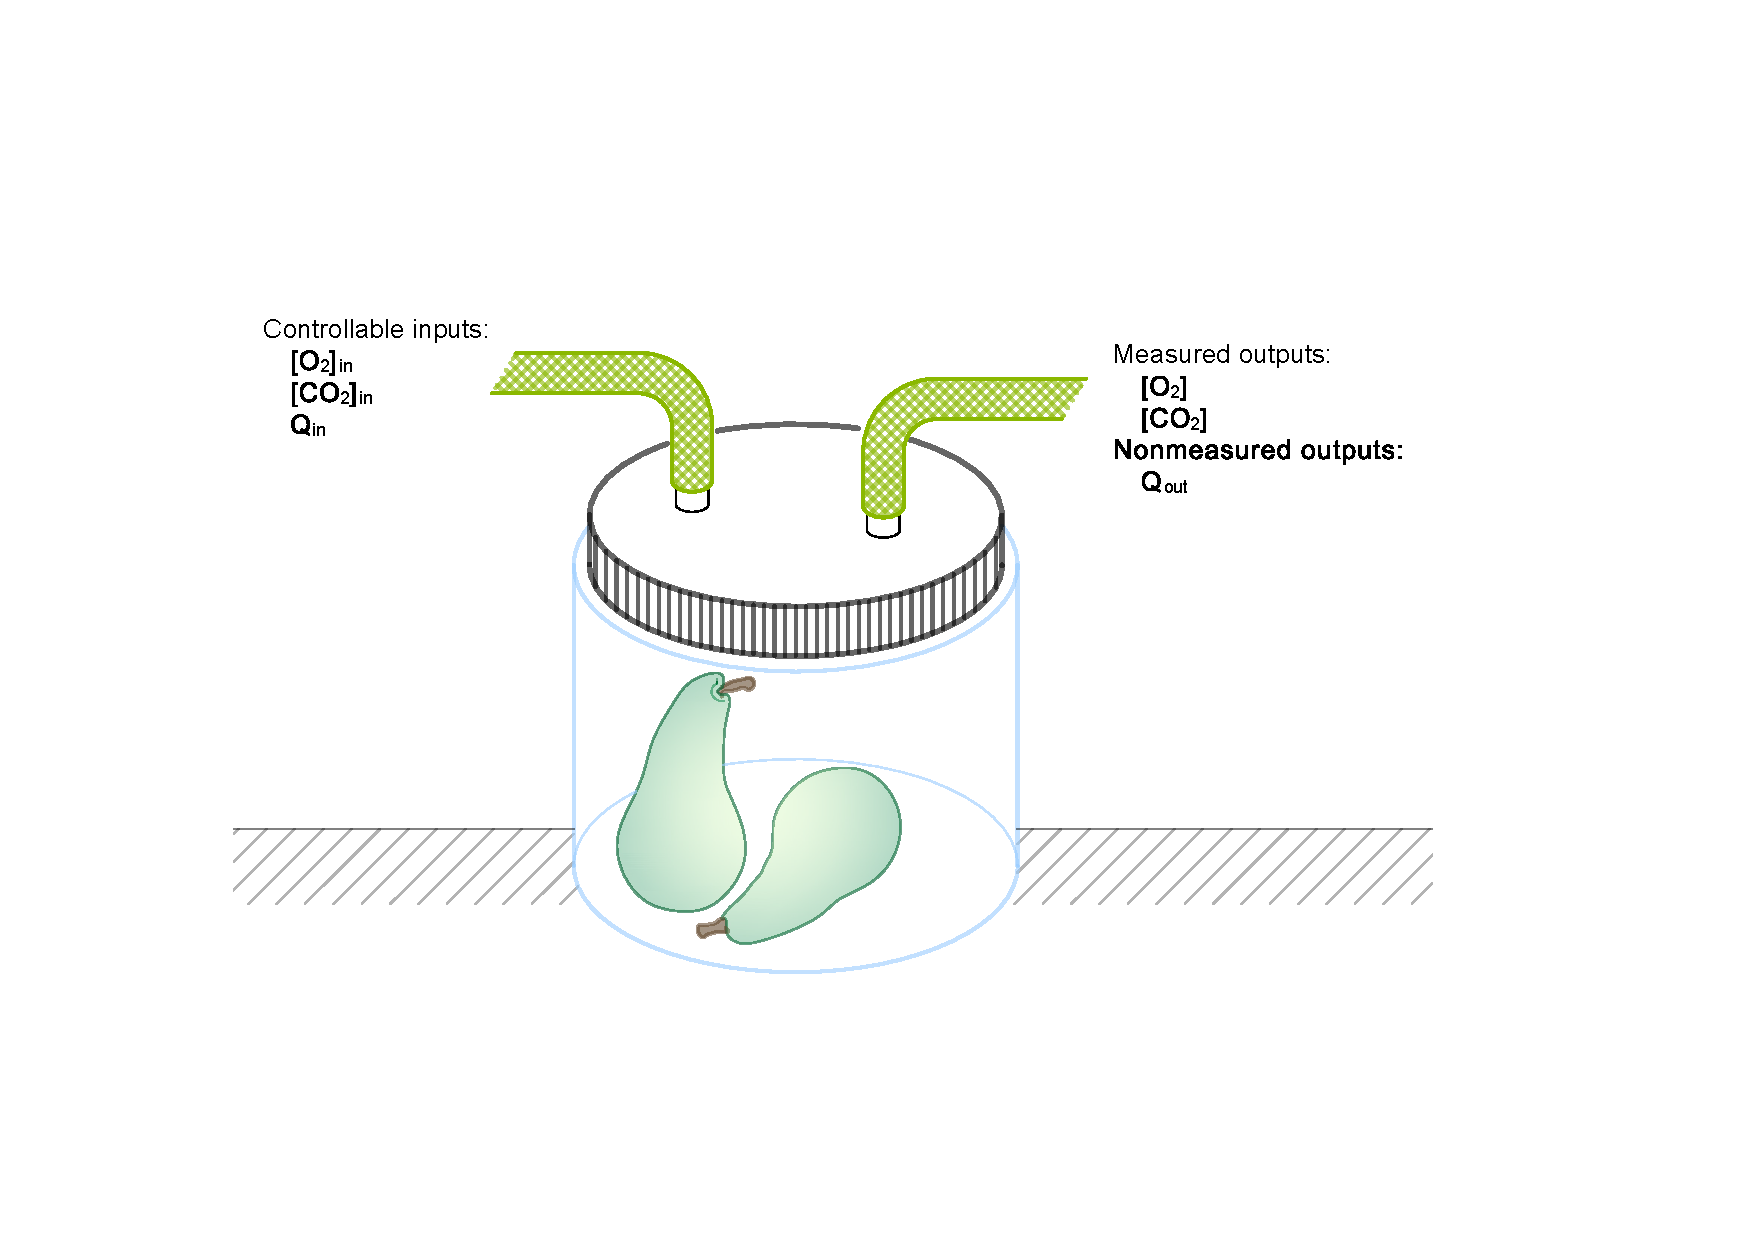
\includegraphics[width=0.9\textwidth,trim={2cm 4cm 2cm 5cm,clip}]{figure/paper 2/pear.pdf}
	\caption{Schematic representation of the measurement setup.}
	\label{figpear}
\end{figure}
\label{sec_model}
The respiration and fermentation of pear fruit inside a jar is modeled by two mass balances for $\oxy$ and $\coxy$:
\begin{equation}
\begin{aligned}
V_\text{j}\diff{\Coxy}{t} &= Q_\text{in}(t)\Coxy_{\text{in}}(t) - Q_\text{out}(t)\Coxy
- m_\text{p}r_{\oxy}(t),\\
V_\text{j}\diff{\Ccoxy}{t} &= Q_\text{in}(t)\Ccoxy_{\text{in}}(t) - Q_\text{out}(t)\Ccoxy
+ m_\text{p}r_{\coxy}(t).
\end{aligned}
\label{respiration}
\end{equation}
The square brackets in these expressions represent concentrations in $\text{mol/m}^3$. These differential equations describe the change of $\oxy$ and $\coxy$ concentrations inside a jar with volume $V_j$, which will equal $5\text{ dm}^3$, in our examples in Section \ref{sec_experiments}. A time varying air mixture with an oxygen concentration $\Coxy_{\text{in}}(t)$ and a carbon dioxide concentration $\Ccoxy_{\text{in}}(t)$ is blown into the jar with flow rate $Q_\text{in}(t)$ (units: $\text{m}^3\text{/h}$). These three time varying functions form the controllable inputs to our system. Our measurement set up is schematically shown in Figure \ref{figpear}.
\\
\\
Since the pressure inside the jar should remain equal to the atmospheric pressure, we can calculate the outflow $Q_\text{out}(t)$ from the jar using the ideal gas law:
\begin{equation}
Q_{\text{out}}(t)\frac{P_\text{atm}}{\bar{R}T} = Q_{\text{in}}\frac{P_\text{atm}}{\bar{R}T} - m_p r_{\oxy}(t) + m_p r_{\coxy}(t),
\label{balance}
\end{equation}
with $\bar{R}$ the universal gas constant and $P_\text{atm}$ the atmospheric pressure. Concentrations throughout the jar and at the outlet are considered to be similar, due to the assumption of well mixing. In the constructed experiments in Section \ref{sec_experiments}, the temperature equals $293.15$ K,  the amount of $\oxy$ consumed and $\coxy$ produced is proportional to the mass of the pears $m_\text{p}$, taken to be 4 kg and the initial conditions for $\oxy$ and $\coxy$ will be equal to regular air.
\\
\\
The respiration rates in Equation (\ref{balance}) are specified using models of the Michaelis-Menten type \parencite{hertog}:
\begin{equation}
\begin{aligned}
r_{\oxy}(t) &= 
\frac{V_{\text{m},\oxy}\Coxy}
{(K_{\text{m},\oxy} + \Coxy)
	(1 + \frac{\Ccoxy}{K_{\text{mn},\text{CO}_2}})},\\
r_{\coxy}(t) &= 
\text{r}_\text{q}r_{\oxy}(t) + 
\frac{V_{\text{m,f,}\coxy}}
{1 + \frac{\Coxy}{K_{\text{m,f},\oxy}}}.
\end{aligned}
\end{equation}
The models for these respiration rates contain six parameters that have to be identified. $V_{\text{m},\oxy}$ and $V_{\text{m,f,}\coxy}$ are the maximum respiration and fermentation reaction rates, respectively. The Michaelis-Menten constant $K_{\text{m},\text{O}_2}$ represents the saturation of respiration at high oxygen levels, whereas $K_{\text{mn},\text{CO}_2}$ models the inhibition of respiration by $\coxy$. The respiration quotient $\text{r}_\text{q}$ represents the percentage of $\oxy$ that is converted to $\coxy$ by respiration. Finally, $K_{\text{m,f},\oxy}$ models the inhibition of fermentation by $\oxy$.
\\
\\
The measured gas concentrations $\Coxy_m$ and $\Ccoxy_m$ at time point $t_k$ are assumed to be equal to the true concentrations plus the additive Gaussian noise terms $\zeta_k$ and $\eta_k$ respectively:
\begin{equation}
\begin{aligned}
\Coxy_{m}(t_k) &= \Coxy(t_k) + \zeta_k,\\
\Ccoxy_{m}(t_k) &= \Ccoxy(t_k) + \eta_k.
\end{aligned}
\end{equation}
Since both measurements are in the same range from $0$ to $30\text{ kPa}$, we assume that the error terms are identically and independently distributed for both outputs, and thus that variance, $\sigma^2$, of the error terms $\zeta_k$ and $\eta_k$ is equal.
\subsection{Prior Information}
Optimal experimental design for the non-linear model introduced in Section \ref{sec_model} requires prior information, concerning the six respiration and fermentation parameters. Such prior information for pear respiration and fermentation can be found in \textcite{ho}. We cannot directly utilize the published results, as \textcite{ho} only report confidence intervals for each individual parameter, but no correlations between estimates. To deal with this problem, we reanalyzed $50$ time series data-sets, each containing $\oxy$ and $\coxy$ measurements from a single jar, made available to us by the authors. We used a Bayesian data analysis technique to achieve this. More specifically, we utilized a Markov-chain Monte-Carlo method to re-estimate the parameters and quantify the uncertainty in the data  \parencite{betancourt}. The Markov-chain stores values sampled from the posterior distribution of the parameters. The chain can thus be utilized for numerically approximating the expectation in the robust criterion in Equation (\ref{pseudoD}). In other words, we use the MCMC chain as an input to the expression in Equation (\ref{pseudoDcalc}).
\\
\\
Because the data of \textcite{ho} were collected at different temperatures, our analysis took into account the effect of temperature on the maximal respiration and fermentation rate by means of the Arrhenius equations:
\begin{equation}
\begin{aligned}
V_{\text{m},\oxy} &=
V_{\text{m},\oxy,T_r}\exp\left(E_{a,\oxy}\left ( \frac{1}{T_r} - \frac{1}{T} \right) \right),\\
V_{\text{m,f,}\coxy} &= V_{\text{m,f,}\coxy,T_r}\exp\left(E_{a,\coxy}\left (\frac{1}{T_r} - \frac{1}{T} \right)\right),
\end{aligned}
\end{equation}
where $V_{\text{m},\oxy,T_r}$ and $V_{\text{m,f,}\coxy,T_r}$ are the maximal respiration rates at a reference temperature $T_r$ of $293.15$ K, and $E_{a,\oxy}$ and $E_{a,\coxy}$ are activation energies that describe how the reaction rates increase with the temperature $T$. These activation energies are nuisance parameters in our computation of optimal input profiles in Section \ref{sec_experiments}, as we only consider experiments at the reference temperature.
\\
\\
Figure \ref{figprior} provides a summary of the results of our Bayesian analysis. On the diagonal of this figure, histograms of the Markov-chain values of the six model parameters of interest ($V_{\text{m},\oxy}$, $K_{\text{m},\oxy}$, $K_{\text{mn},\text{CO}_2}$, $r_q$, $V_{\text{m,f,}\coxy}$, $K_{\text{m,f},\oxy}$) are shown. Below the diagonal, two-dimensional heatmaps are shown, which visualize the correlation between the Markov chain values for pairs of model parameters. The figures above the diagonal provide similar information, but show only $100$ pairs of values from the Markov-chain. Histograms of the Markov chain values for the nuisance parameters $E_{a,\oxy}$, $E_{a,\coxy}$, and $\sigma$ are depicted in Figure \ref{fignuisance}.
\begin{sidewaysfigure}[ht]
	\centering
	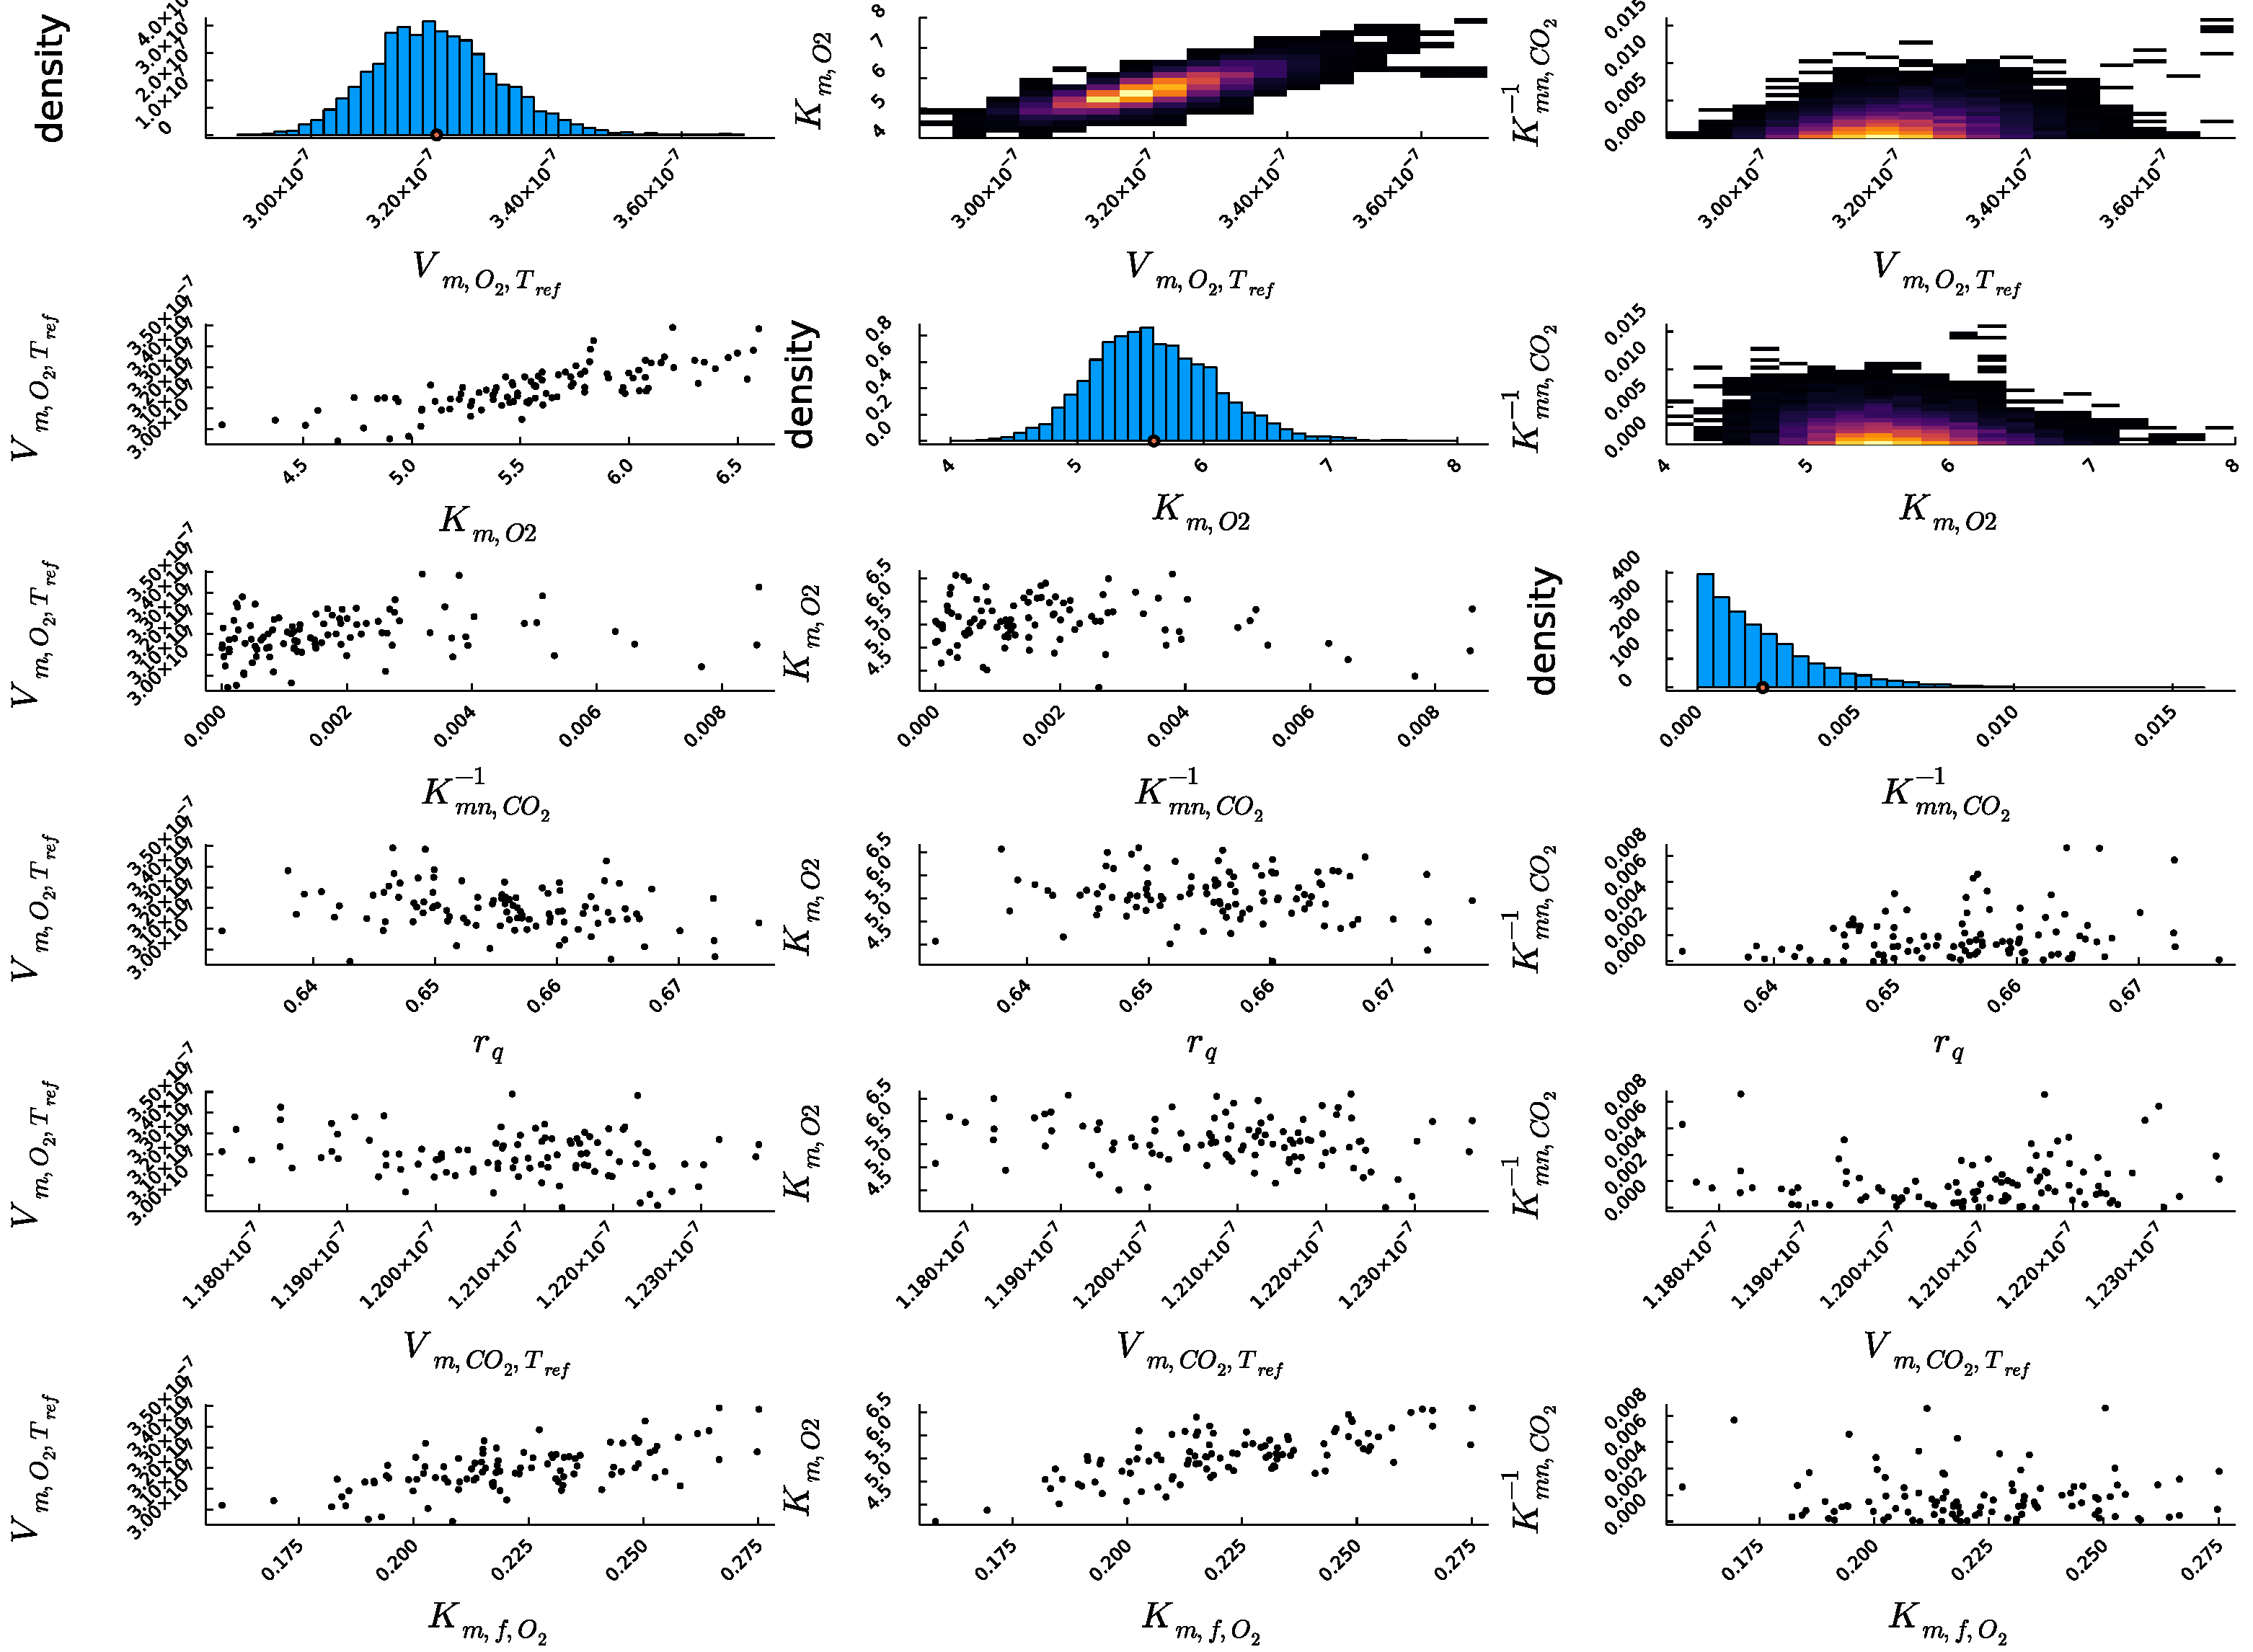
\includegraphics[width=0.9\textwidth]{figure/paper 2/test.pdf}
	\caption{Summary of the Bayesian data analysis of the data in \textcite{ho} for the parameters of interest.}
	\label{figprior}
\end{sidewaysfigure}
\clearpage
The estimation of the respiration inhibition parameter, $K_{\text{mn},\text{CO}_2}$, from the available data was problematic. For this reason, we had to reparametrize the model using the inverse of $K_{\text{mn},\text{CO}_2}$. As can be seen in the third histogram in Figure \ref{figprior}. $K_{\text{mn},\text{CO}_2}^{-1}$ takes values close to zero, which means $K_{\text{mn},\text{CO}_2}$ tends to infinity. The lack of information about $K_{\text{mn},\text{CO}_2}^{-1}$ can be explained as follows: to precisely estimate this parameter, both high $\oxy$ and $\coxy$ concentrations are needed. A high $\oxy$ concentration is required because otherwise there is no respiration that can be inhibited, and a high $\coxy$ concentration is required because otherwise the inhibition has a negligible effect. Data points in which both gasses posses a high concentration do not occur in the data of \textcite{ho}. $K_{\text{m,f},\oxy}$ is the second hardest parameter to identify, from the data of \textcite{ho}, because the $\oxy$ concentration needs to be in a specific range for this parameter to have an effect on the outputs. An $\oxy$ concentration much higher than $K_{\text{m,f},\oxy}$ means no fermentation is happening at all, and an $\oxy$ concentration much lower than $K_{\text{m,f},\oxy}$ implies maximal fermentation. The third most difficult parameter to identify is  $K_{\text{m},\text{O}_2}$, because the model is only sensitive to this parameter when $\oxy$ concentrations are close to the value of this parameter.
\begin{figure}[H]
	\centering
	\begin{subfigure}[b]{0.3\textwidth}
		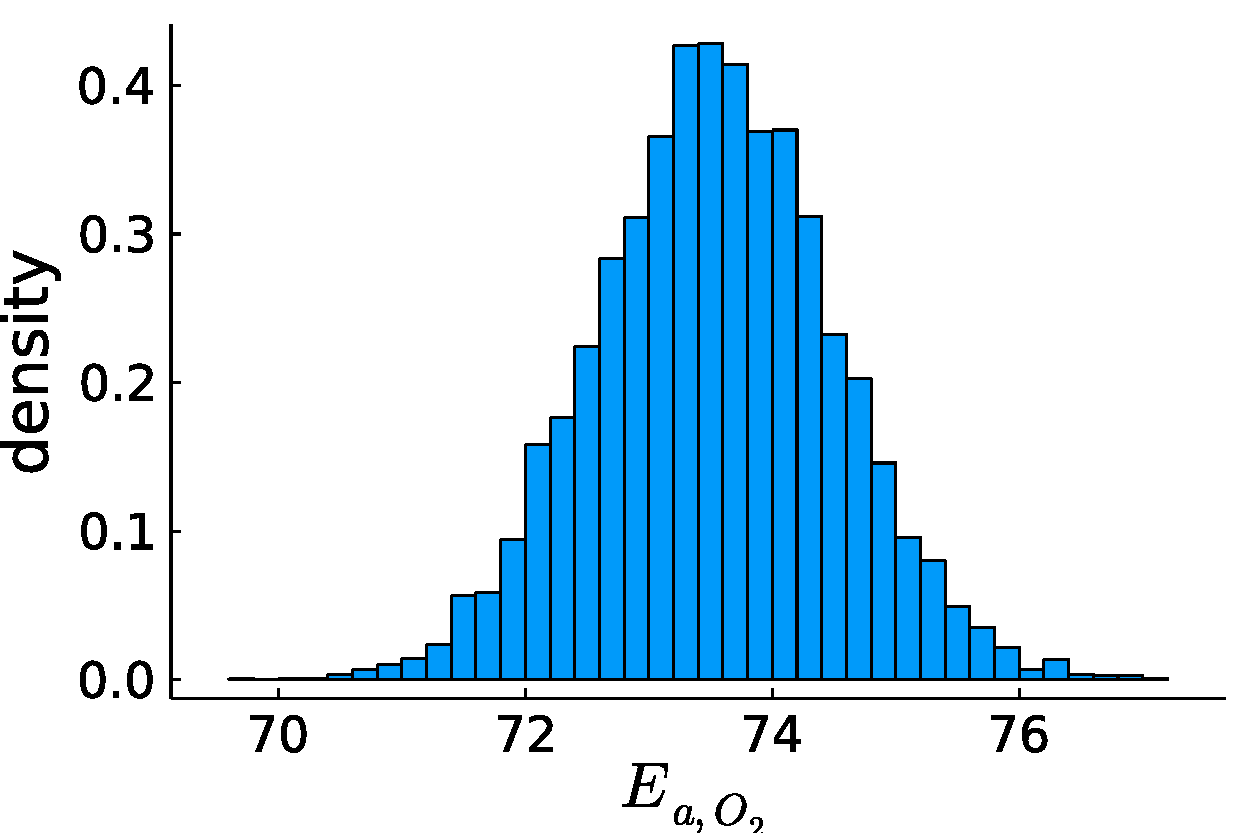
\includegraphics[width=1.0\textwidth]{figure/paper 2/nuisance1.pdf}
	\end{subfigure}
	\begin{subfigure}[b]{0.3\textwidth}
		\centering
		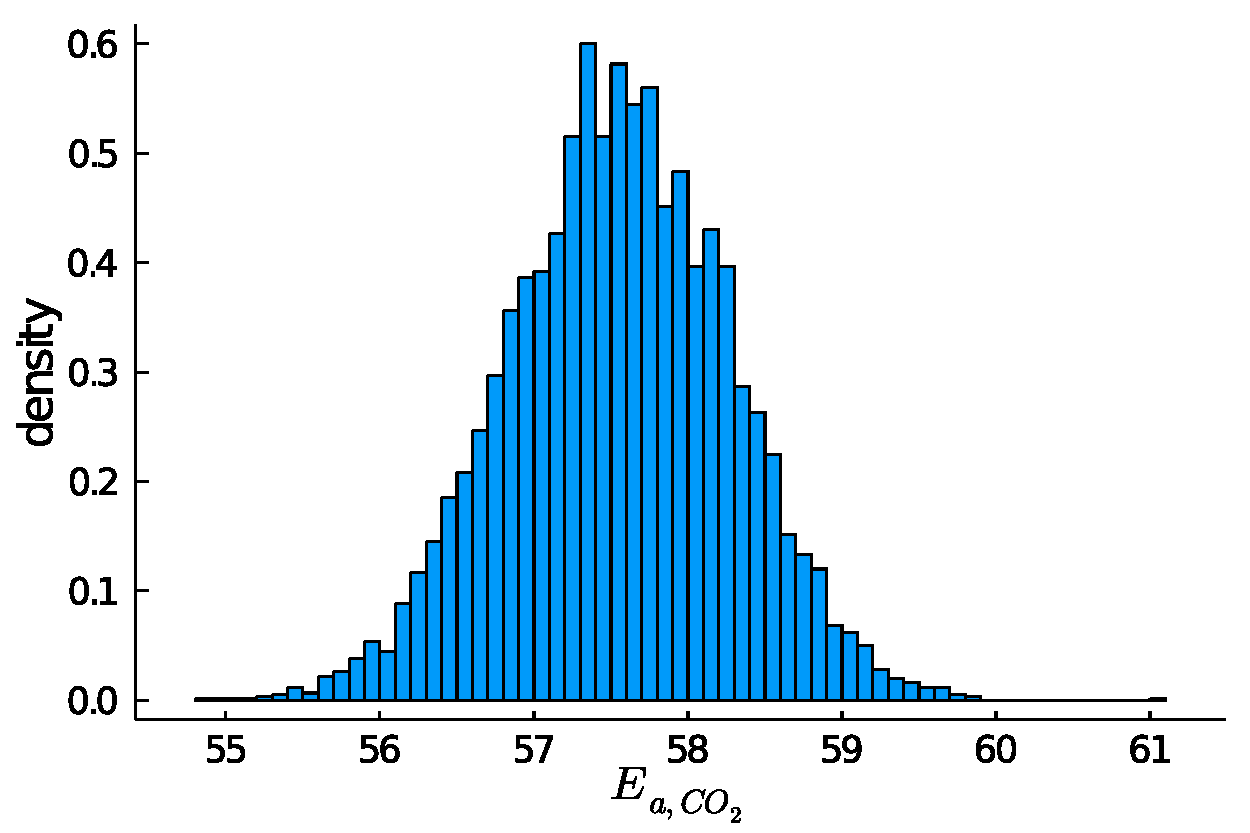
\includegraphics[width=1.0\textwidth]{figure/paper 2/nuisance2.pdf}
	\end{subfigure}
	\begin{subfigure}[b]{0.3\textwidth}
		\centering
		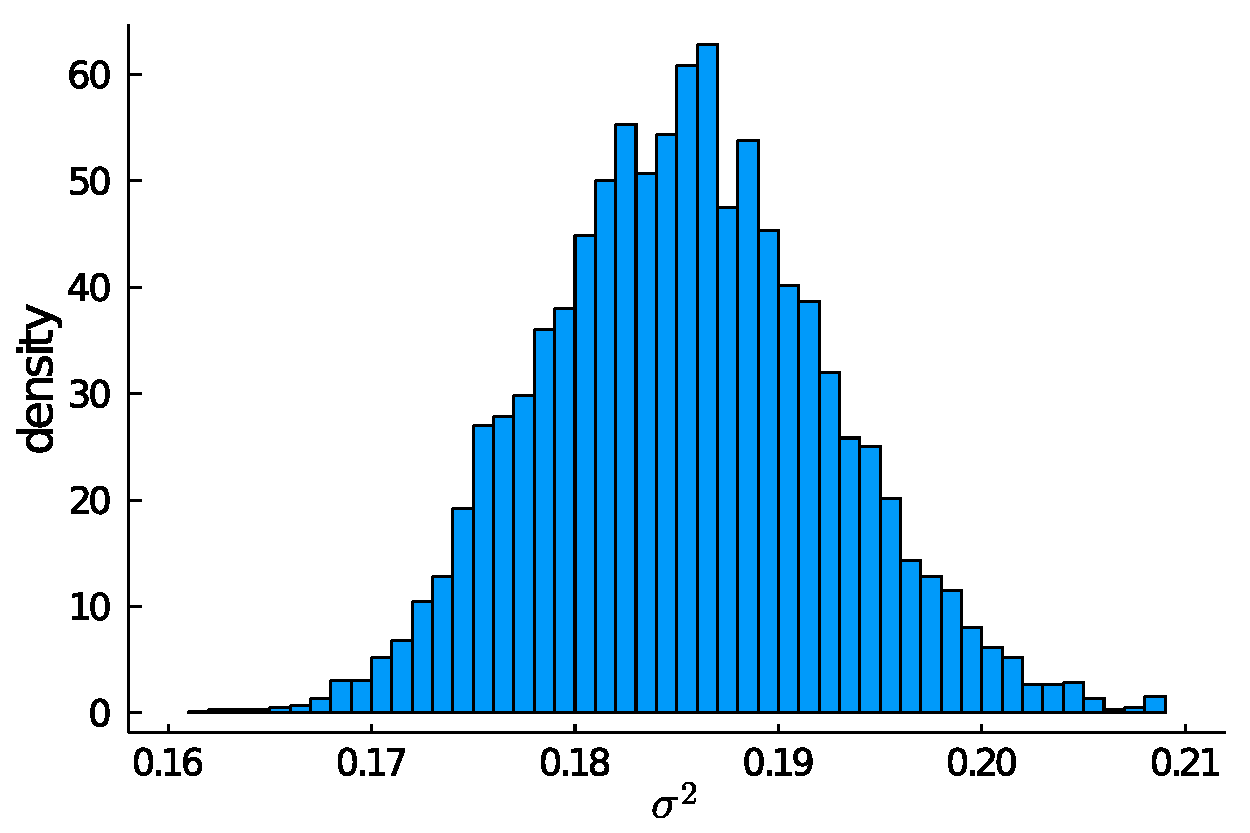
\includegraphics[width=1.0\textwidth]{figure/paper 2/nuisance3.pdf}
	\end{subfigure}
	\caption{Summary of our Markov-chain Monte-Carlo analysis of the data in \textcite{ho} for the nuisance parameters $E_{a,\oxy}$, $E_{a,\coxy}$ and $\sigma^2$.}
	\label{fignuisance}
\end{figure}
\subsection{Markov-chain Details}
\label{sec_markov}
The data analysis was performed using the No U-Turn Sampling Markov-chain Monte-Carlo algorithm \parencite{hoffman}, as implemented in Turing.jl \parencite{ge}. We ran 4 parallel Markov chains each starting from the maximum likelihood estimates of the parameters, and each chain comprises 1500 steps. We utilized a flat prior in the physically possible regions of the unknown parameters. For all parameters this means that only positive values are possible, with $r_q$ being at most $1$.
\\
\\
We used the posterior distribution resulting from this Bayesian analysis of the experiments in \textcite{ho} as a prior distribution for the generation of the robust designs in this chapter. However, as calculating Bayesian optimal designs with the entire Markov chain is numerically quite intensive, we discarded the first 500 step, and thinned the remaining 1000 by a factor 40. This gave us 100 samples to calculate the Bayesian D-optimality criterion in Equation (\ref{pseudoD}). These are also the 100 values shown in the top right half of Figure \ref{figprior}.
\section{Results}
\label{sec_experiments}
In our examples, we consider experiments lasting $24$ h with measurements taken every $5$ minutes, i.e. $t_e = 24$ h and $N=288$. The maximum and minimum flow rates are equal to $1\text{ l h}^{-1}$ and $0.1\text{ l h}^{-1}$, respectively. The input gas concentrations are allowed to vary between $0 \text{ kPa}$ and $21\text{ kPa}$. We did not use a minimum flow rate of $0\text{ l h}^{-1}$, because at zero flow there is no difference in system response between a maximal or minimal gas input concentration. This implies that the design selection criteria from Equations (\ref{localD}) and (\ref{pseudoDcalc}) are flat in certain directions, causing numerical issues for gradient based optimizers. Working with a strictly positive minimum flow rate avoids this issue.
\subsection{Locally Optimal Designs for the Respiration and Fermentation Model}
We take the average values of the Markov chains of the parameters of interest, as well as the average of the Markov chain values of the parameter $\sigma^2$ to evaluate the local D-criterion in Equation (\ref{pseudoD}). These values are shown in Table \ref{tableLocal}, and indicated by a bullet in the histograms on the diagonal of Figure \ref{figprior}. We start by analyzing the effect of an increasing refinement of the discretization of the inputs $\bm u(t)$. In Figure \ref{figconvergence}, which shows the local D-criterion value as a function of the number of times the input signal is allowed to switch, we see that the D-criterion no longer improves noticeably after $M = 48$, which corresponds to a switch every half hour. The experimental design obtained with $M = 12$, which corresponds to a switch every two hours, already performs well. Therefore, in the remainder of this chapter, we consider $\oxy$, $\coxy$ and flow rate inputs that remain constant for two-hour time periods.
\begin{table}[h!]
	\centering
	\setlength{\tabcolsep}{4pt} 
	\small
	\begin{tabular}{|c c c c c c c|}

		\hline
		$V_{\text{m},\oxy}$ & $K_{\text{m},\oxy}$ &  $K_{\text{mn},\text{CO}_2}$ & $r_q$ & $V_{\text{m,f,}\coxy}$ & $K_{\text{m,f},\oxy}$ & $\sigma^2$\\ [0.5ex] 
		\hline
		$\mu$mol$\text{ kg}^{-1}$ $\text{ s}^{-1}$ & kPa & kPa & - & $\mu$mol$\text{ kg}^{-1}$ $\text{ s}^{-1}$& kPa & $\text{mol}^2$$\text{ m}^{-6}$	\\ [0.5ex] 
		\hline
		0.320 & 5.61 & 484.4 & 0.655 & 0.121 & 0.224 & 0.186\\ [1ex] 
		\hline
	\end{tabular}
	\caption{Parameters used for the optimization of the construction of the locally optimal designs.}
	\label{tableLocal} 
\end{table}
\begin{figure}[H]
	\centering
	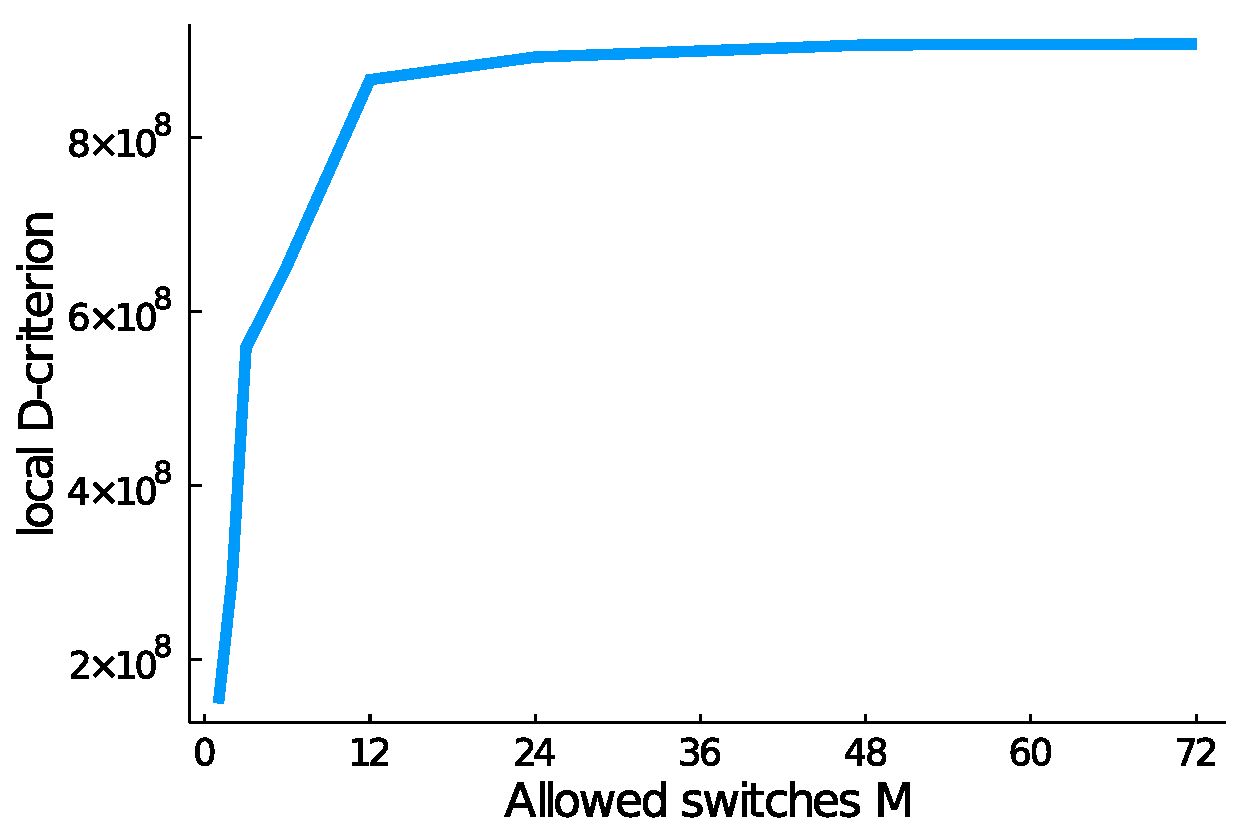
\includegraphics[width=0.9\textwidth]{figure/paper 2/convergence.pdf}
	\caption{Convergence of the local D-optimality criterion for finer discretizations of the controls.}
	\label{figconvergence}
\end{figure}
The locally optimal design for the scenario in which the inputs are allowed to vary every two hours is shown in more detail in Figures \ref{figlocala} and  \ref{figlocalb}, together with the simulated outputs in Figure \ref{figlocalc}, evaluated at the values of the model parameters used to optimize the design. During the interval from $2$ h to $4$ h, both $\oxy$ and $\coxy$ are pumped into the jar, which causes high concentrations of the two gasses to be present at the same time. We noted before that, due to the lack of such conditions in \textcite{ho}, it was impossible to estimate $K_{\text{mn},\text{CO}_2}$ well from their data. However, the $\oxy$ concentration cannot remain high throughout the entire experiment, as then there would be insufficient information about non-saturated respiration, i.e. to estimate $K_{\text{m}, \oxy}$ precisely. The $\oxy$ concentration must decrease further to levels at which fermentation starts to occur for $K_{\text{m,f},\oxy}$ to become estimable. This explains why air, with zero $\oxy$ inlet concentrations is pumped into the jar in the interval between $10$ h and $12$ h. The $\coxy$ inlet concentration is also zero during that time interval due to the fact that the $\coxy$ concentration is not allowed to run up too high, as this compromises the ability to precisely determine the fermentation parameters. This can be intuitively understood by considering the system in an extreme scenario where the atmosphere in the jar consists entirely of $\coxy$. In this scenario, the outflow will also be pure $\coxy$ regardless of the values of the fermentation parameters. Information about the fermentation parameters is then only incorporated in the outflow rate, but this is not a measured output. This illustrates how optimal experiments automatically take into account the specifics of the measurement setup.  The pumping action at $18$ h, again involving zero $\oxy$ and $\coxy$ concentrations, is performed for similar reasons.
\begin{figure}[H]
	\centering
	\begin{subfigure}[b]{0.45\textwidth}
		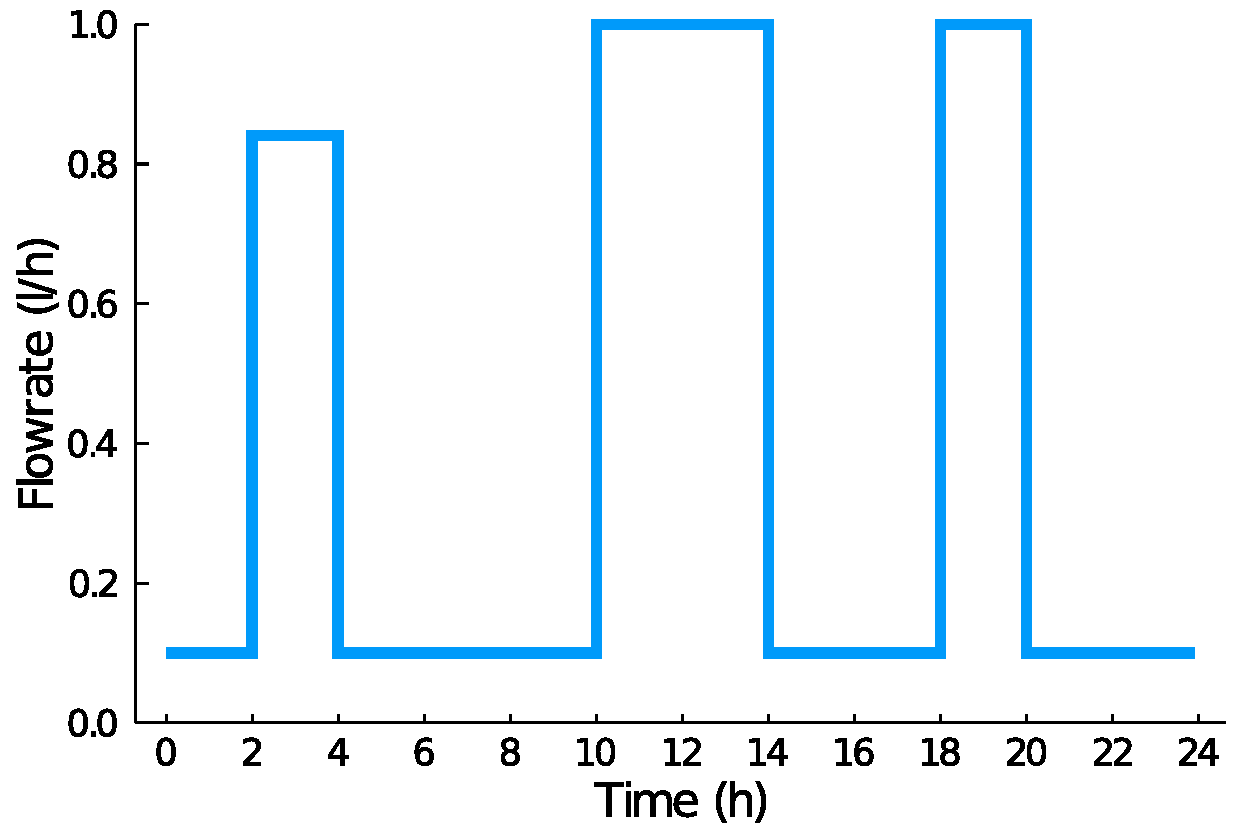
\includegraphics[width=1.0\textwidth]{figure/paper 2/l12_input_flow.pdf}
		\caption{Input flow.}
		\label{figlocala}
	\end{subfigure}
	\begin{subfigure}[b]{0.45\textwidth}
		\centering
		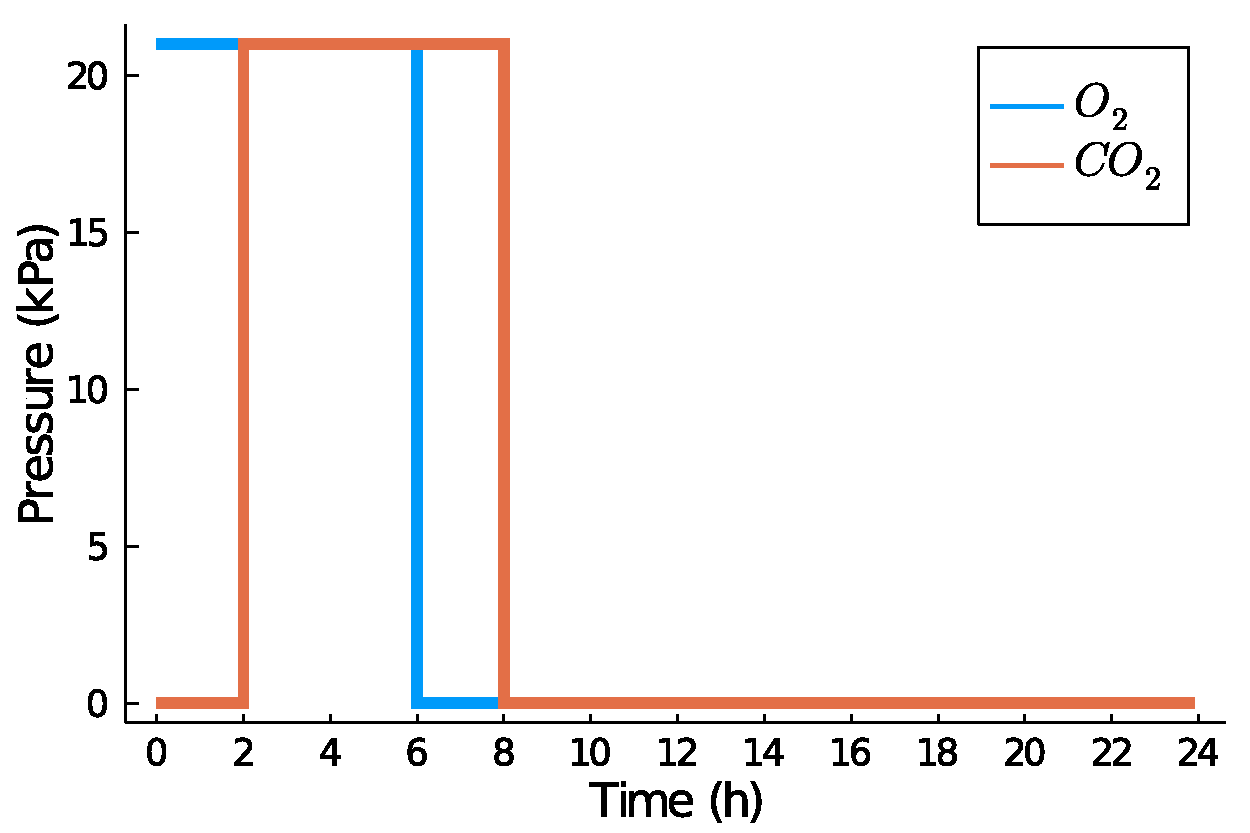
\includegraphics[width=1.0\textwidth]{figure/paper 2/l12_input_gass.pdf}
		\caption{Input gasses.}
		\label{figlocalb}
	\end{subfigure}
	\\
	\begin{subfigure}{0.45\textwidth}
		\centering
		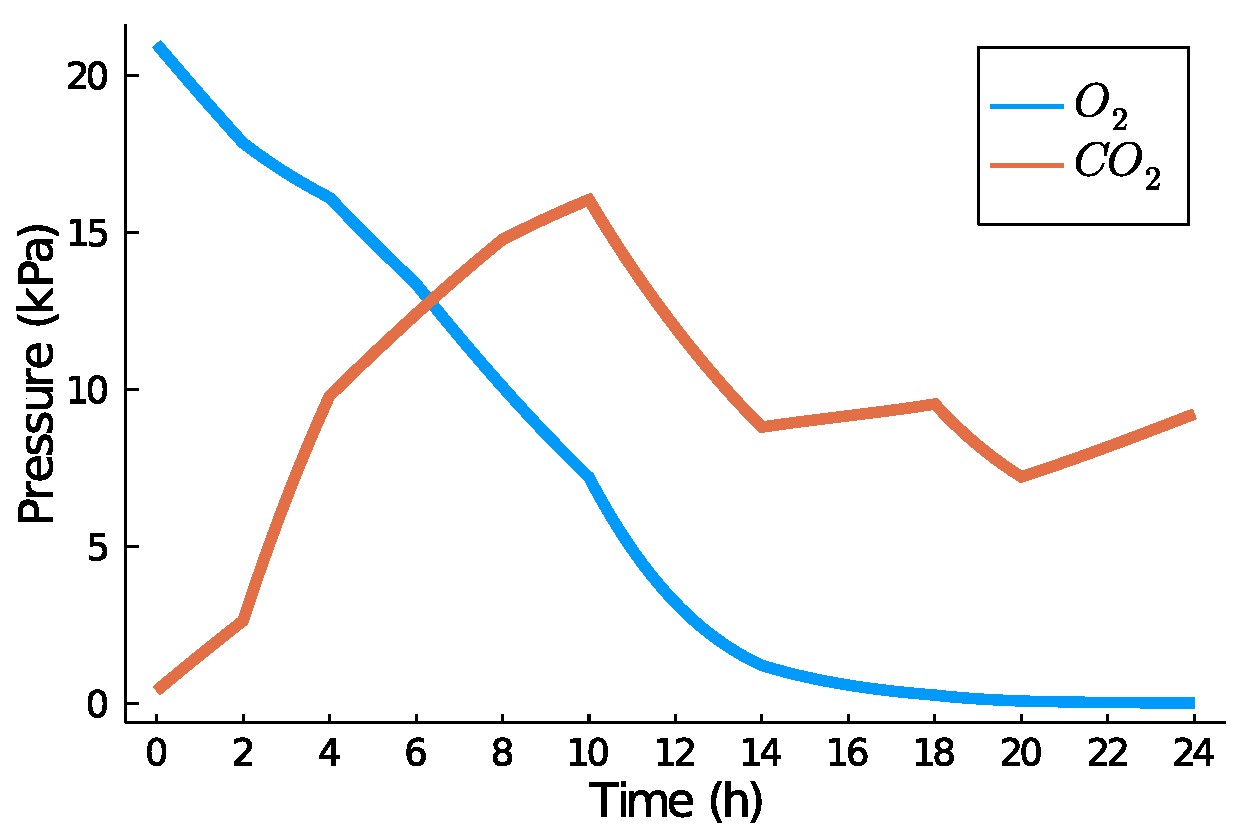
\includegraphics[width=1.0\textwidth]{figure/paper 2/l12_output.pdf}
		\caption{Output gasses.}
		\label{figlocalc}
	\end{subfigure}
	\caption{Locally optimal experiment and simulated output, with control input switches every two hours.}
	\label{figlocal}
\end{figure}
Figure \ref{figlocald} shows the coefficients of variation of all six model parameters. The three inhibition parameters ($K_{\text{m},\oxy}$, $K_{\text{mn},\text{CO}_2}$ and $K_{\text{m,f},\oxy}$) remain the most difficult to estimate ones. Now, however, in our experiment involving a single jar, instead of using the data from $50$ jars, made available to us by \textcite{ho}, the model parameters can be estimated much more precisely.
\begin{figure}[H]
	\begin{subfigure}[b]{0.45\textwidth}
		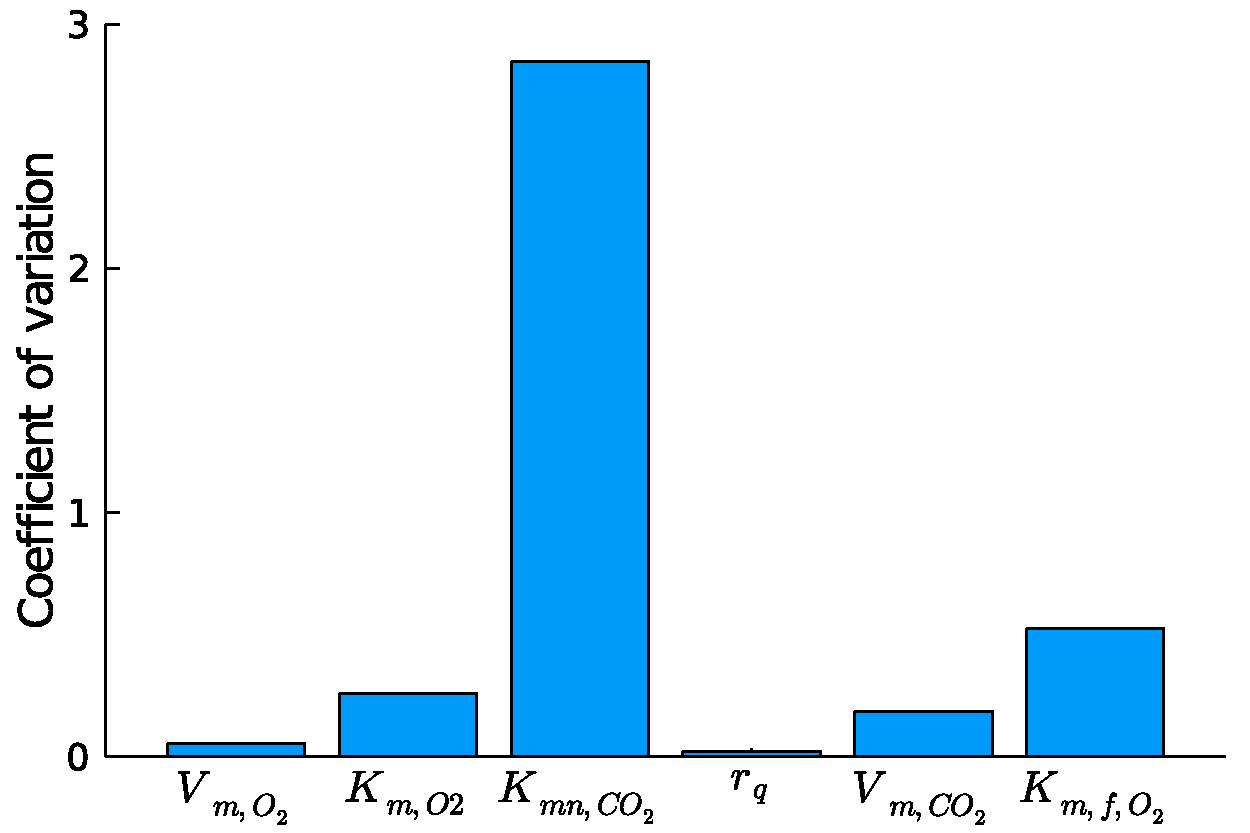
\includegraphics[width=1.0\textwidth]{figure/paper 2/l12_var.pdf}
		\caption{coefficients of variation}
		\label{figlocald}
	\end{subfigure}
	\begin{subfigure}[b]{0.45\textwidth}
		\centering
		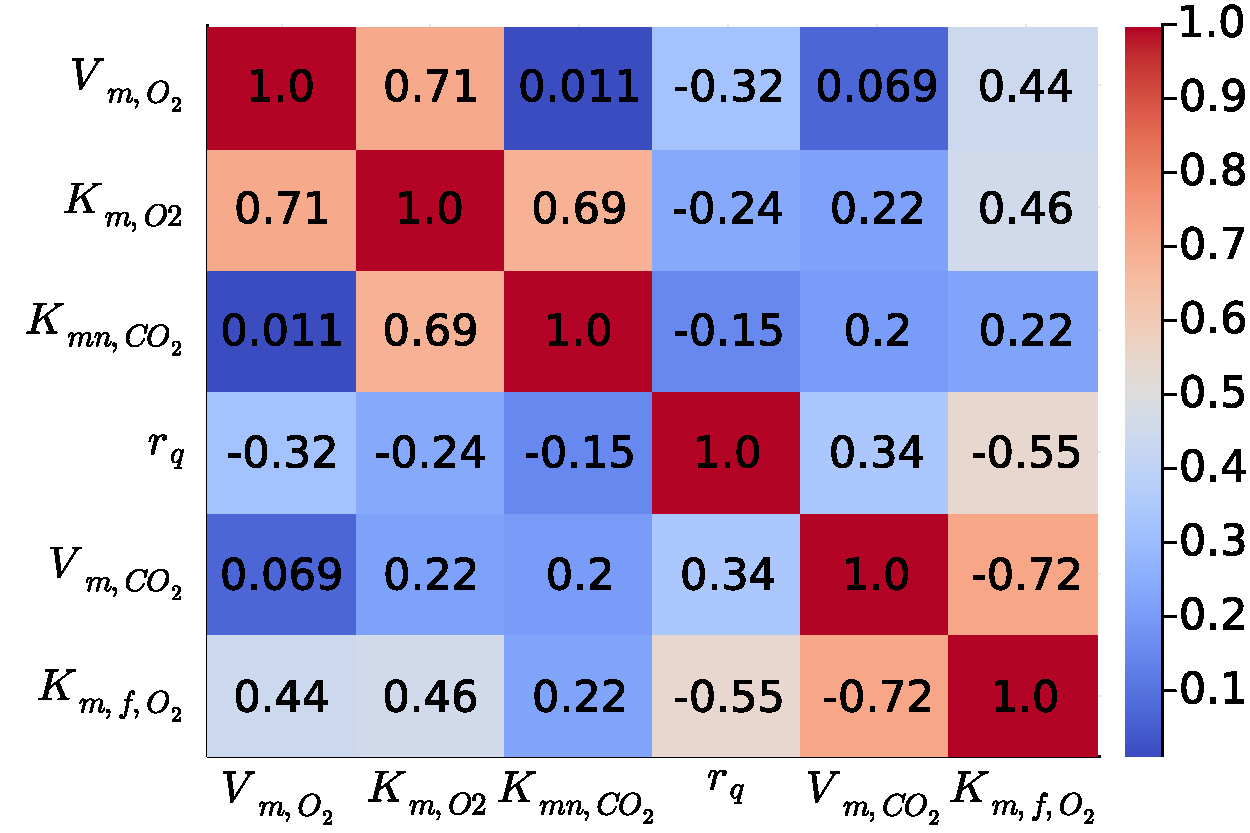
\includegraphics[width=1.0\textwidth]{figure/paper 2/l12_corr.pdf}
		\caption{absolute value of correlations}
		\label{figlocale}
	\end{subfigure}
	\caption{Summary of the information gained from the locally optimal experiment in Figure \ref{figlocal}.} 
\end{figure}
Figure $\ref{figlocale}$ shows a map of the absolute values of the correlations of the estimates that would be obtained if the locally optimal experiment were to be used. Because there are no strong correlations between the first three parameters and the last three parameters, we can thus visualize the FIM in Equation (\ref{FIM}) using two ellipsoids. More specifically, we can use one ellipsoid to show the gain in information for the parameters $V_{\text{m},\oxy}$, $K_{\text{m},\oxy}$, and $K_{\text{mn},\text{CO}_2}$ and another ellipsoid to show the gain in information for the parameters $\text{r}_\text{q}$, $V_{\text{m,f,}\coxy}$ and $K_{\text{m,f,}\oxy}$. These ellipsoids are shown in Figures \ref{figlocalf} and \ref{figlocalg} for the experiment allowing changes in inputs every two hours, compared to an experiment that only allows inputs to be set at the start of the experiment ($M=1$ in Equation (\ref{input})). This is indicated in red, for the optimal experiment that allows switches every two hours, and indicated in blue, for the optimal experiment when the inputs must remain constant throughout the entire experiment. The volume of the ellipsoids of the experiment allowing more switches is smaller.
\begin{figure}[H]
	\begin{subfigure}[b]{0.45\textwidth}
		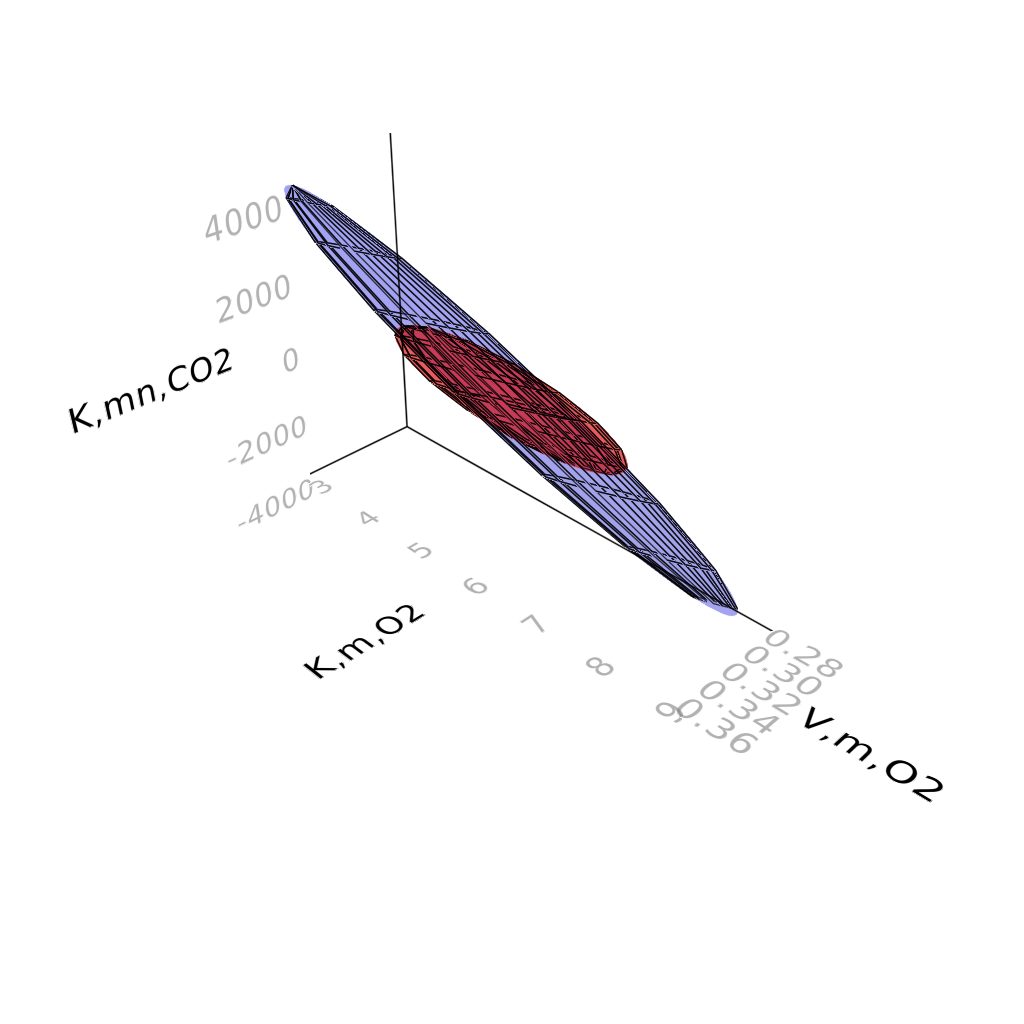
\includegraphics[width=1.0\textwidth]{figure/paper 2/ellipsoid1_3.png}
		\caption{first three parameters ($V_{\text{m},\oxy}$, $K_{\text{m},\oxy}$, $K_{\text{mn},\text{CO}_2}$).}
		\label{figlocalf}
	\end{subfigure}
	\begin{subfigure}[b]{0.45\textwidth}
		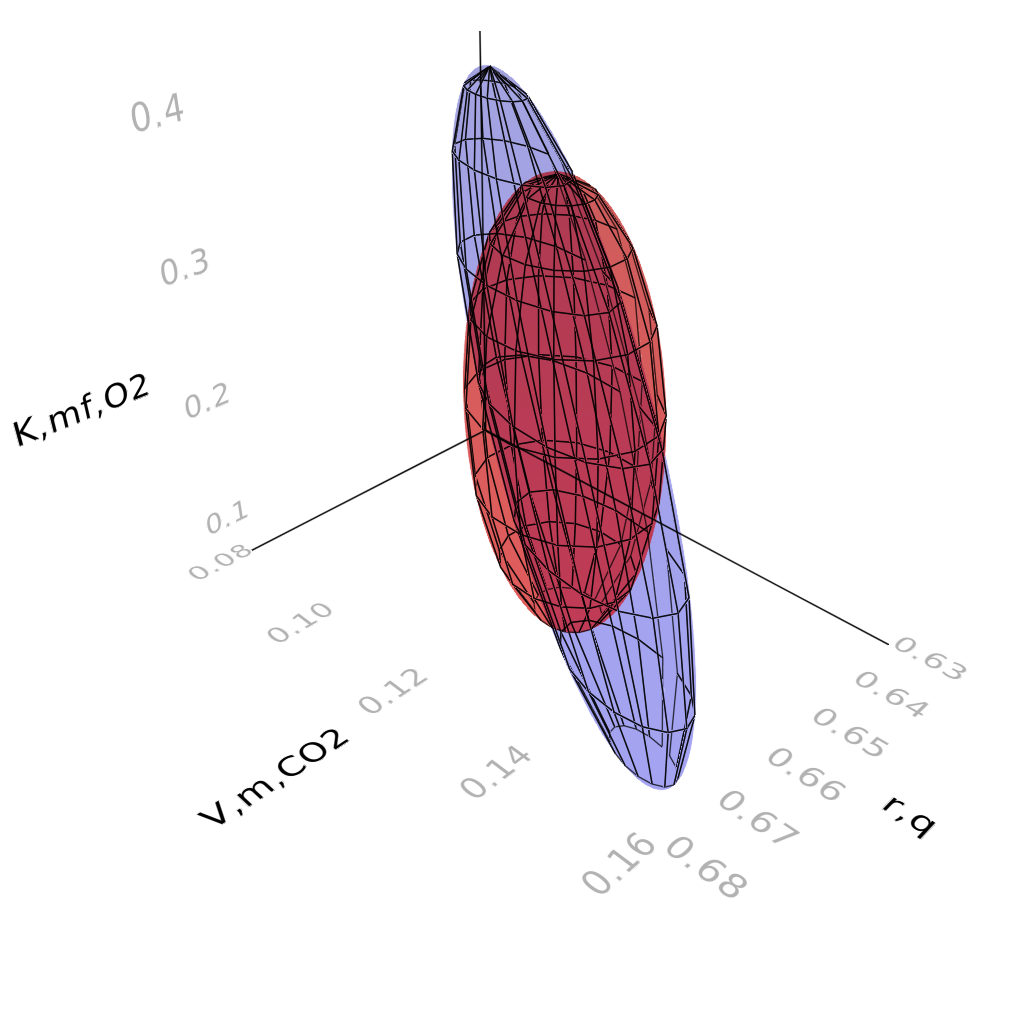
\includegraphics[width=1.0\textwidth]{figure/paper 2/ellipsoid4_6.png}
		\caption{last three parameters ($r_q$, $V_{\text{m,f,}}$, $K_{\text{m,f},\oxy}$).}
		\label{figlocalg}
	\end{subfigure}
	\caption{95\% confidence ellipsoids comparing $M=12$ (red) and $M=1$ (blue).} 
	\label{figellipsoid}	
\end{figure}
\subsection{Bayesian Optimal Designs for the Respiration and Fermentation Model}
We now continue by searching a more robust design than the locally optimal design in Figure \ref{figlocal}. Instead of optimizing the determinant of the FIM in Equation (\ref{FIM}) for the means of the Markov-chain values, we optimize the mean determinant for a thinned version of the Markov chain. These values are graphically shown by the blue bullets in the upper right hand part of Figure \ref{figprior}. The design found by maximizing the robust optimality criterion in Equation (\ref{pseudoDcalc}) is shown in Figures \ref{figbayesiana} and \ref{figbayesianb}. The simulated output for all values of the thinned Markov chain is shown in Figure \ref{figbayesianc}. The robust design exhibits several similarities to the locally optimal design, but also some key differences. The occurrence of a pumping action in the time interval between $2$ h and $4$ h as well as the interval between $10$ h and $14$ h is similar to that in the locally optimal design in Figure \ref{figlocala}. Furthermore, there are no differences in $\oxy$ and $\coxy$ input concentrations between the robust and locally optimal design. One main difference between the robust experimental design and the locally optimal one is that, in the former, the first pumping action is less intense, i.e. the flow rate only amounts to $0.5$ l$\text{h}^{-1}$, as opposed to  $0.8$ l$\text{h}^{-1}$, in the locally optimal design. A second main difference is the absence of the third pumping action in the robust design. We hypothesize this is because  less pumping actions must occur to ensure a high $\coxy$ concentration when inhibition of respiration by $\coxy$ only happens at high $\coxy$ concentrations, which is possible, since we have little prior knowledge about $K_{\text{mn},\text{CO}_2}$.
\begin{figure}[H]
	\centering
	\begin{subfigure}[b]{0.45\textwidth}
		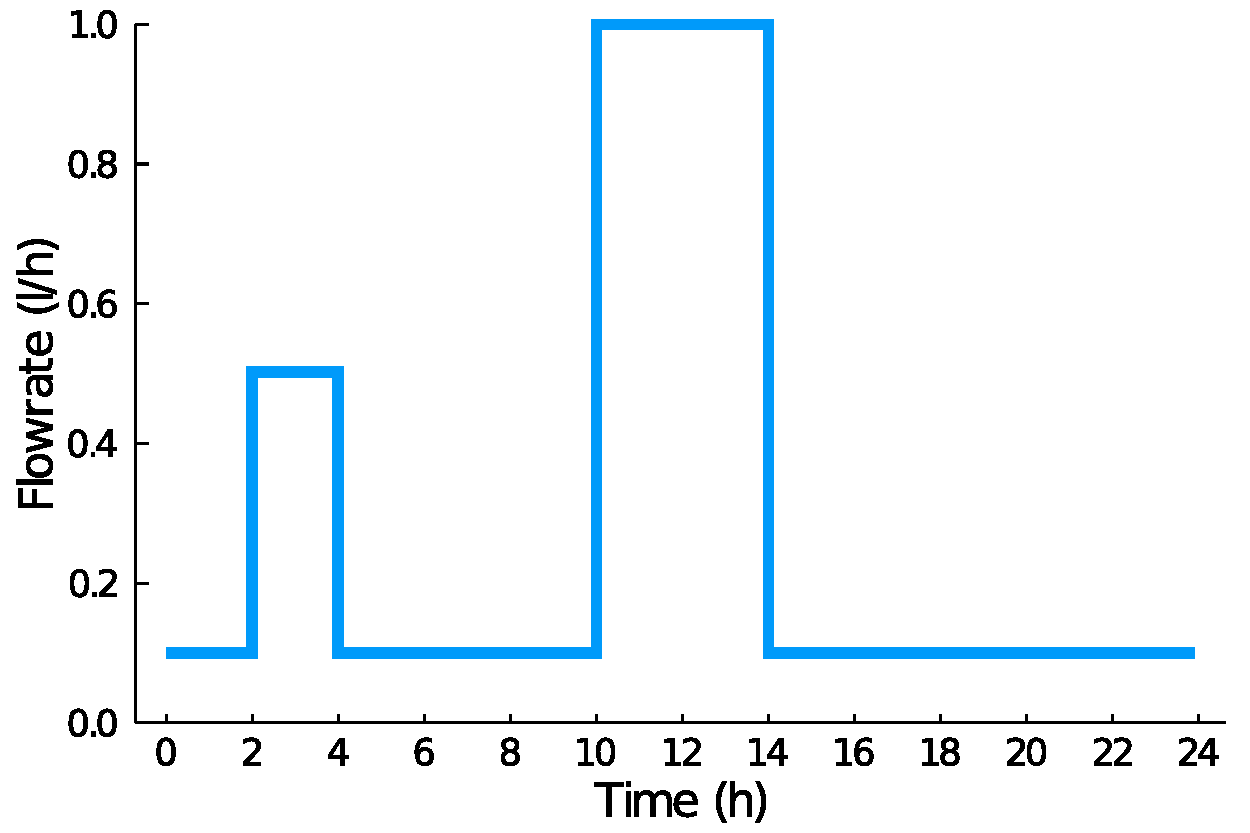
\includegraphics[width=1.0\textwidth]{figure/paper 2/b12_input_flow.pdf}
		\caption{Input flow.}
		\label{figbayesiana}
	\end{subfigure}
	\begin{subfigure}[b]{0.45\textwidth}
		\centering
		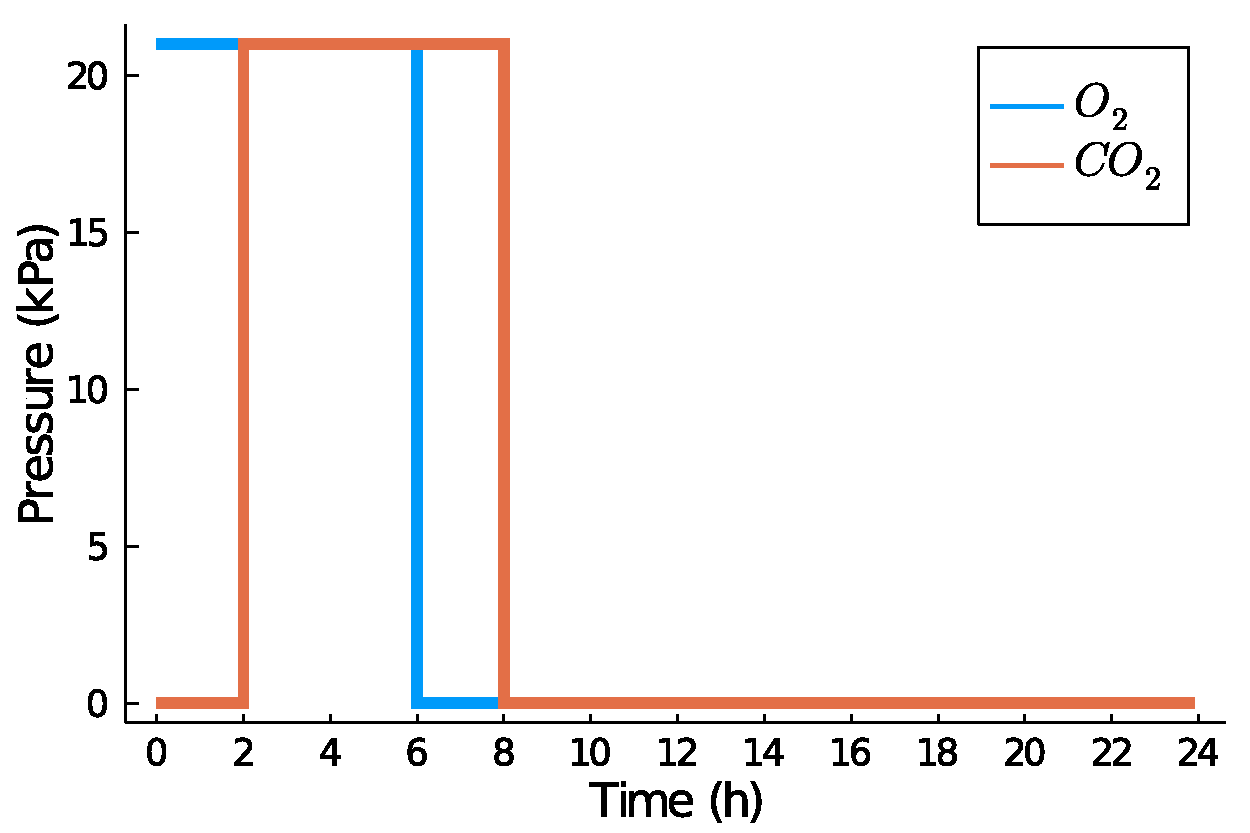
\includegraphics[width=1.0\textwidth]{figure/paper 2/b12_input_gass.pdf}
		\caption{Input gasses.}
		\label{figbayesianb}
	\end{subfigure}
	\\
	\begin{subfigure}{0.45\textwidth}
		\centering
		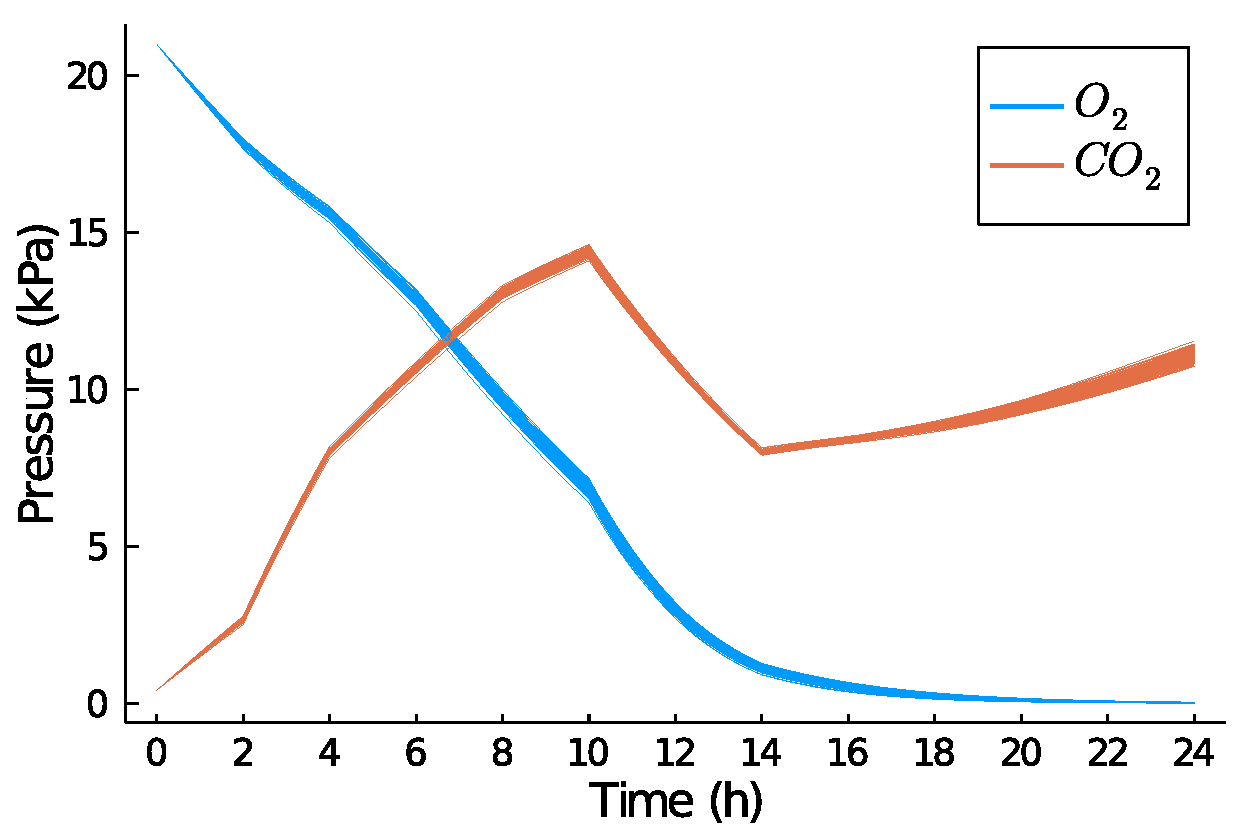
\includegraphics[width=1.2\textwidth]{figure/paper 2/b12_output.pdf}
		\caption{Output, evaluated at each of the model parameter values from the thinned Markov chain.}
		\label{figbayesianc}
	\end{subfigure}
	\caption{Robust optimal experiment and simulated output, obtained using $100$ parameter values from the Markov chain and control input switching every two hours.}
	\label{figbayesian}
\end{figure}
Figure \ref{figbayesianhistogram} shows the difference in performance between the robust and the locally optimal experiment. More specifically, the histogram shows the difference between the determinant of the FIM in Equation (\ref{FIM}) for both the robust and locally optimal design at all $6000$ model parameter values from the Markov chain. For many possible model parameter values, the locally optimal and robust design perform almost equally well. However, the histogram clearly has a heavy right tail, showing that, for some parameter values, the Bayesian design performs significantly better. As the histogram does not posses a heavy left tail, the reverse is not true. The robust design is thus substantially less sensitive to the exact values of the model parameters. It therefore provides better guarantee for a highly informative experiment than the locally optimal design. Since this result holds for the entire Markov chain and not just the thinned version, we can be confident that the thinned version is sufficient to summarize the prior uncertainty, and that the resulting robust design only works well for the specific model parameter values used to evaluate the optimality criterion in Equation (\ref{pseudoDcalc}). Finally, the positive mean value for the difference in determinants, indicated by the orange dot in Figure \ref{figbayesianhistogram}, proves that Bayesian design is expected to do better for the region of prior uncertainty.
\begin{figure}[H]
	\centering
	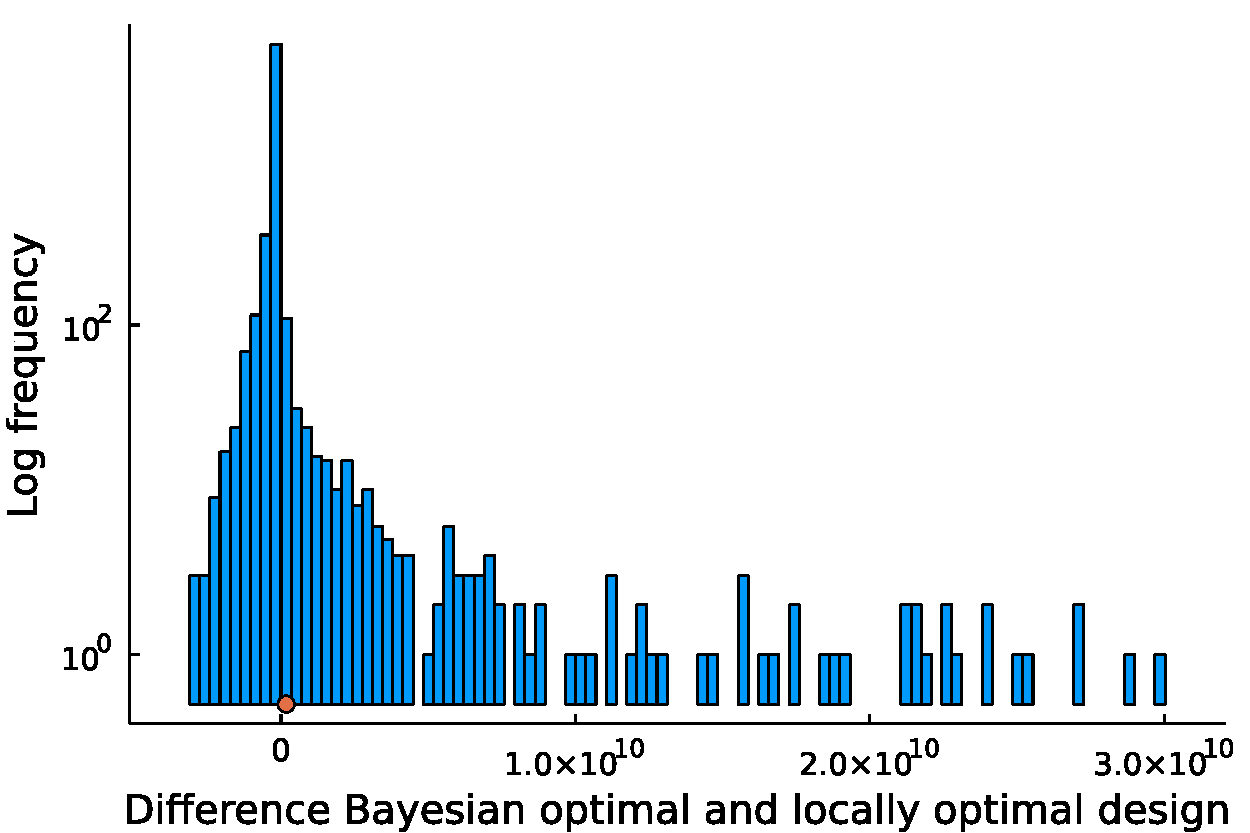
\includegraphics[width=0.9\textwidth]{figure/paper 2/histogram.pdf}
	\caption{Histogram of difference in determinants of the FIM of the robust and locally optimal designs for $6000$ parameters from the prior distribution. Positive values mean the robust design performs better.}
	\label{figbayesianhistogram}
\end{figure}
\section{Discussion and Future Work}
\label{sec_discussion}
\subsection{Alternative Information Criteria}
In this chapter, we presented a robust experimental design methodology for dynamic models and applied that methodology to precisely estimate the respiration and fermentation parameters of fruit and vegetables. We achieved this by quantifying the information content of the experiments using the determinant of the Fisher information matrix averaged out over a prior distribution, represented by a Markov chain. Another possible approach would be to quantify information based on the expected Kullback-Leibler divergence (KL-div) between the prior and posterior distributions \parencite{lindley}. For larger experiments, the expected KL-div is asymptotically equal to our Bayesian D-optimality criterion. For small experiments, the KL-div approach might be superior as it does not utilize normal approximations. One major downside of using the KL-div is its computational complexity, as it involves calculating a high dimensional integral over all possible outcomes $\bm y $ of the experiment. This is generally done using a double loop Monte-Carlo integration method \parencite{ryan}. Some research has been done using this method for determining optimal sampling times of dynamic systems \parencite{overstall2}, but this work does not consider optimal control. Therefore, the dynamic system in  \parencite{overstall2} does not need to be  solved repeatedly for different control actions. Instead, only a single dynamic system needs to be solved that can be evaluated at different possible sampling times. Selection of input profiles based on the KL-div is considered in \textcite{liepe}, but only for a small  discrete set of possible input profiles. In contrast, in this chapter, we optimize the experimental design over a large continuous space of possible experimental designs. Recently, advances have been made in lowering the computational burden of the KL-div based approach by considering variational Bayesian techniques \parencite{foster}, where the inner Monte-Carlo loop is replaced by optimizing a variational distribution. This technique then allows for jointly optimizing the design and variational parameters \parencite{foster2}. In future work, we will employ these variational Bayesian techniques for adaptive dynamic experiments, where the design is modified online as data is collected.
\subsection{State Discretization}
In this chapter, we discretized only the controls $\bm u$, but not the states $\bm x$. The discretization of states is applied using multiple shooting and collocation based dynamic optimization approaches \parencite{biegler}. Generally, these methods lead to optimization problems that are faster to solve, but which might lead to poorer designs. Besides the faster computing time, one additional reason to consider discretization of the states would be the presence of additional constraints on the states. This is because violations of such constraints are difficult to check without a discretization. Our optimization problem did not involve any such additional state constraints. \textcite{nimmegeers} provide a more detailed discussion on the incorporation of constraints into optimal dynamic experiments.
\subsection{Reverse Automatic Differentiation}
We used forward mode automatic differentiation to calculate the sensitivities to the unknown parameters $\bm \theta$, required to obtain the FIM in Equation (\ref{FIM}), and this was further nested to calculate the gradient of the D-criteria in Equations (\ref{localD}) and (\ref{pseudoDcalc}) with respect to the control parameters $\bm u$. Forward mode automatic differentiation generally performs well for functions with a small number of inputs, relative to the number of outputs. For our respiration model, it thus was a good choice for calculating the unknown parameter sensitivities present in the FIM. Reverse mode automatic differentiation performs better for functions with many more outputs than inputs. It thus seems like a natural choice to calculate the gradients necessary for the optimization of the control parameters. However, there is currently not yet a mature implementation of reverse over forward mode automatic differentiation in the Julia ecosystem \parencite{rackauckas2}.
\section{Conclusion}
This chapter presented a pioneering study about the usefulness of robust optimal dynamic experiments for non-linear modeling in postharvest research. Robust designs work well for a range of possible model parameter values. Robust design methods require the specification of a prior distribution for the model parameters. Current methods in the literature only work for parametric prior distributions. The available prior information about respiration and fermentation of pear fruit could not be adequately summarized using a parametric distribution, thus we developed a novel experimental design methodology based on a Markov-chain Monte-Carlo analysis of a prior data-set. This Markov chain can approximate arbitrary distributions. We used this methodology to construct robust D-optimal dynamic experimental designs for the estimation of the Michaelis-Menten respiration and fermentation parameters of Conference pear were constructed. These robust designs perform better than locally D-optimal designs, which are optimized using a single initial guess for the model parameters.